%part3.tex

\part{\LaTeX{} 图形命令的使用}

\section{水平间距和居中}\label{sec:center}

\subsection{水平居中}\label{ssec:hcenter}
图形的放置位置由当前文本的排列方式所决定。
为使图形居中放置,可将其放入居中环境 \env{center} 中。
\begin{lstlisting}
\begin{center}
\includegraphics[width=2in]{graphic.eps}
\end{center}
\end{lstlisting}

如果 \cmd{includegraphics} 命令处于一个环境中
(例如 \env{minipage} 或 \env{figure}),
用 \cmdi{centering} 可将其后的内容居中排列。
例如:

\begin{lstlisting}
\begin{figure}
\centering
\includegraphics[width=2in]{graphic.eps}
\end{figure}
\end{lstlisting}
效果类似于
\begin{lstlisting}
\begin{figure}
\begin{center}
\includegraphics[width=2in]{graphic.eps}
\end{center}
\end{figure}
\end{lstlisting}
这里推荐使用~\cmd{centering},因为~\verb+\begin{center}+~会使图形上下
方的垂直间距增加一倍
( \env{figure} 带有的垂直间距加上 \env{center} 环境带有的垂直间距)。
若希望有额外的垂直间距,可使用第~\ref{ssec:vspace}~节介绍的命令。

\cmd{psfig} 和 \cmd{epsfbox} 命令
\marginpar{过时的用法}
的缺陷让它们很难使图形居中排列。
过去,作为一种解决办法,使用了 \TeX{} 命令 \cmdi{centerline} 和 \cmdi{leavevmode}。
而 \cmd{includegraphics} 命令已克服了这些缺陷,
允许直接与 \cmd{centering} 命令一起使用或用在 \env{center} 环境中,
因此也就不需再使 \cmd{centerline} 和 \cmd{leavevmode}了。

\subsection{水平间距}\label{ssec:hspace}
\LaTeX{} 在排列图形的时候实际上与排列其它的像文字这样的对象是一样的,
了解到这一点很重要。
举例来说,如果行尾不是以 \texttt{\%} 结束的话,
\LaTeX{} 会自动在两行之间加进一个字符的水平间距。
例如,
\begin{lstlisting}
Hello
World
\end{lstlisting}
在输出结果中``Hello'' 和 ``World'' 之间会有一个字符的水平间距。
类似地,
\begin{lstlisting}
\includegraphics{file}
\includegraphics{file}
\end{lstlisting}
则在图形之间有一个字符的水平间距。
在第一行的行尾加上注释符\texttt{\%}
\begin{lstlisting}
\includegraphics{file}%
\includegraphics{file}
\end{lstlisting}
就会取消图形之间的水平间距。

如果需要水平间距,可用 \cmdi{hspace} 命令在图形之间
加入指定长度
\footnote{
	用 \cmd{textwidth} 或 \texttt{em} (原文误作 \cmd{em}——译注)等作为 \cmd{hspace} 的参数,
	而不是采用固定长度,可提高文档的通用性。}
或用 \cmdi{hfill} 加入一个可填充可能的间距的弹性长度。
例如:
\begin{lstlisting}
\includegraphics{file.eps}\hfill\includegraphics{file.eps}
\end{lstlisting}
将两个图形尽量向左右分开。而
\begin{lstlisting}
\hspace*{\fill}\includegraphics{file.eps}%
\hfill\includegraphics{file.eps}\hspace*{\fill}
\end{lstlisting}
使得图形的两边和中间的间距都相等。
由于断行前的 \cmd{hfill} 命令会被忽略,
所以需要用\cmdM{hspace*}{\cmd{fill}} 来替代它。

除了 \cmd{hspace} 和 \cmd{hfill} 之外,
\marginpar{其它间距命令}
\cmdi{quad} 命令会插入当前字体大小的空白。
例如,如果使用 \texttt{10 pt} 字体大小,那么 \cmd{quad} 会插入 10 \texttt{pt} 的水平间距。
而命令 \cmdi{qquad} 会插入两倍于 \cmd{quad} 的水平间距。


\section{旋转、缩放和对齐}\label{sec:rotate-scale-align}

\subsection{高度和整体高度的区别}\label{ssec:diffheight}

使用 \opt{height} 选项时必须要小心,
因为用户经常想要的其实是由 \opt{totalheight} 选项设置的整体高度
(参见~\pageref{fig:samplebox} 页的图~\ref{fig:samplebox})。
当对象的深度为零时,对象的整体高度就是它的高度,
此时使用 \opt{height} 选项不会有什么问题。
但是,当对象的深度不为零时,使用 \opt{height} 而不是 \opt{totalheight} 会导致不正确的图像大小或除零的错误。
导入图像时,区分 \opt{height} 和 \opt{totalheight} 对于旋转和缩放时显得尤其重要。
例如:
\begin{lstlisting}
\includegraphics[angle=-45,totalheight=1in]{file}
\includegraphics[angle=-45,height=1in]{file}
\end{lstlisting}
第一个命令缩放一个旋转了的图形,使其全部高度为~1~英寸。
而第二个命令缩放一个旋转了的图形,使其在参考点以上的部分为~1~英寸高。

\subsection{旋转图形的缩放}\label{ssec:enlarge}
当在插图命令中指定高度或宽度时,这里给出的大小并不是图形的大小,
而是图形的 BoundingBox 的大小。
这点在图形旋转和缩放时很重要。例如:
\begin{lstlisting}
\begin{center}
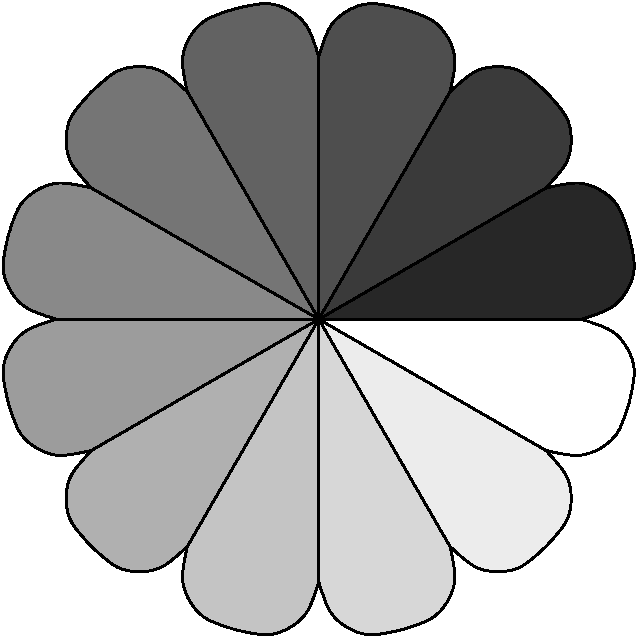
\includegraphics[totalheight=1in]{rosette}
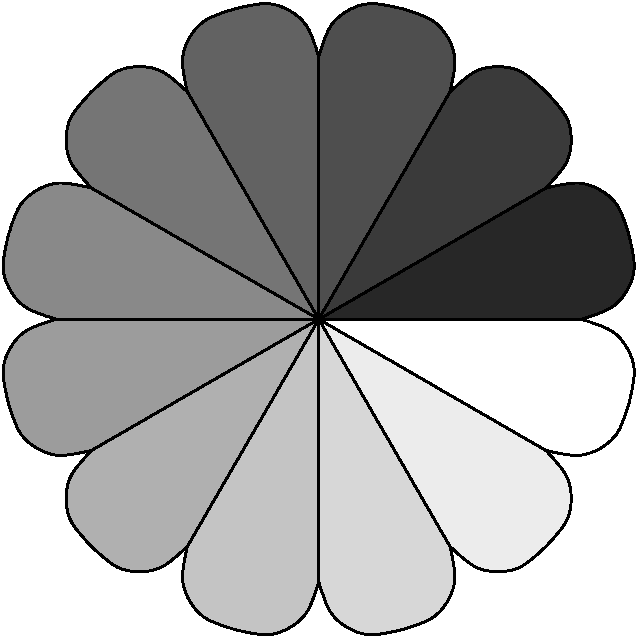
\includegraphics[angle=45,totalheight=1in]{rosette}
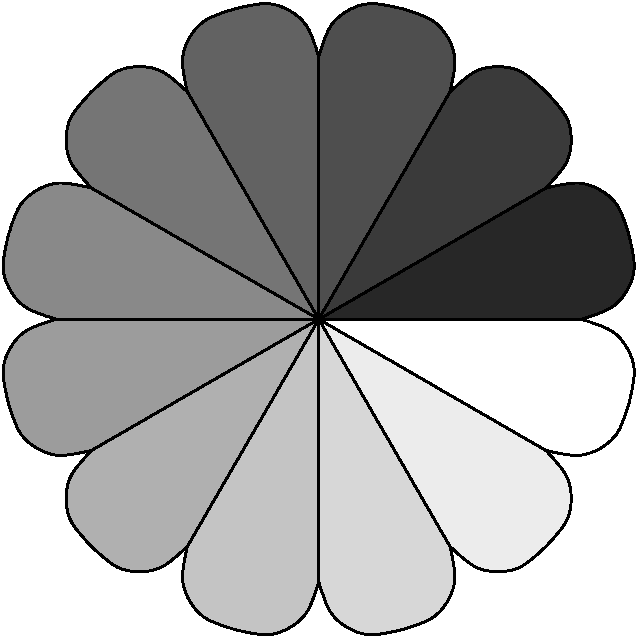
\includegraphics[angle=90,totalheight=1in]{rosette}
\end{center}
\end{lstlisting}
得到

\begin{center}
	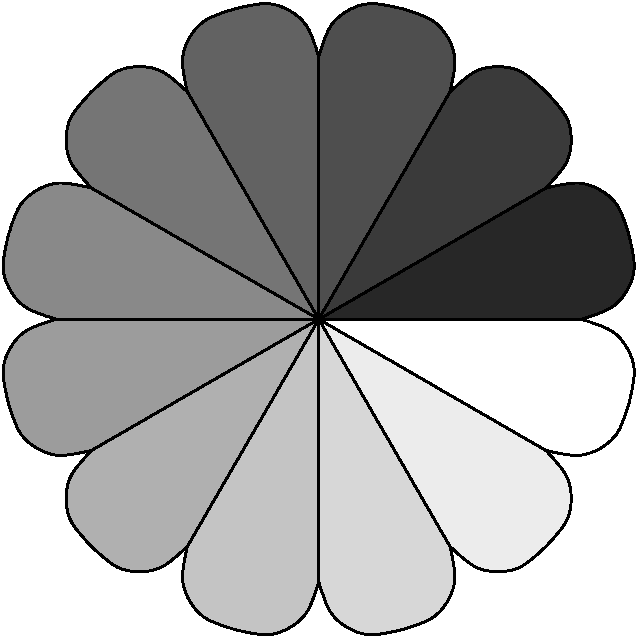
\includegraphics[totalheight=1in]{rosette}
	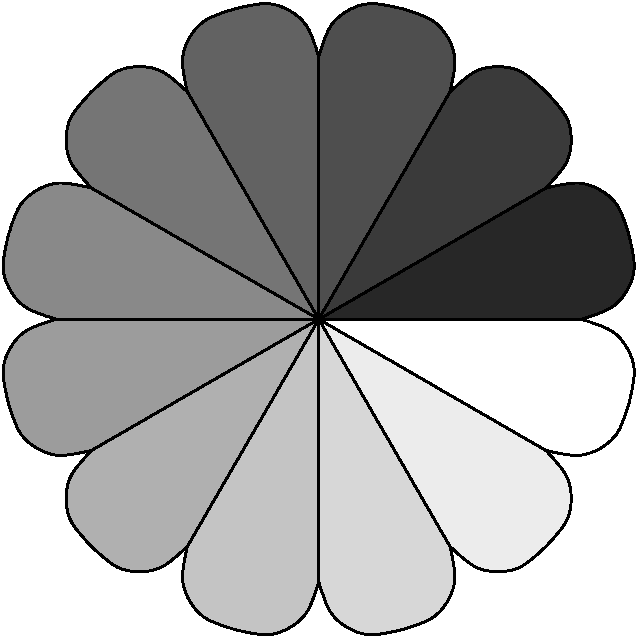
\includegraphics[angle=45,totalheight=1in]{rosette}
	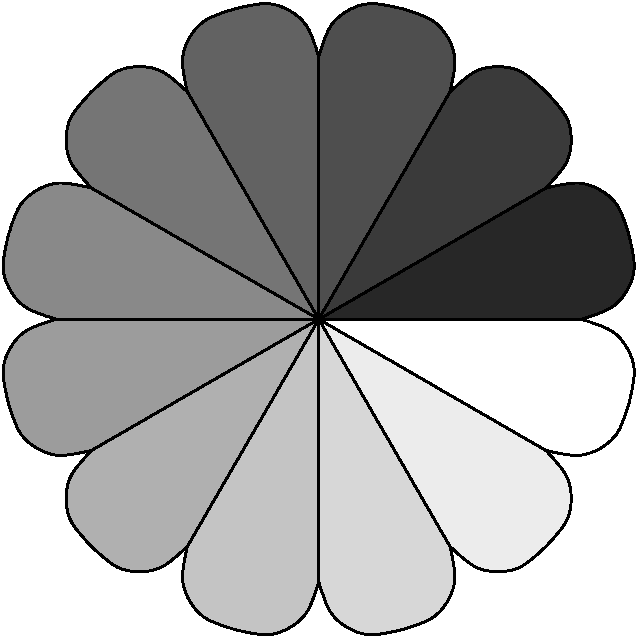
\includegraphics[angle=90,totalheight=1in]{rosette}
\end{center}
尽管看上去图形的大小不一有点奇怪,
但在看过它们的~BoundingBox~后就会明白了。

\begin{center}
	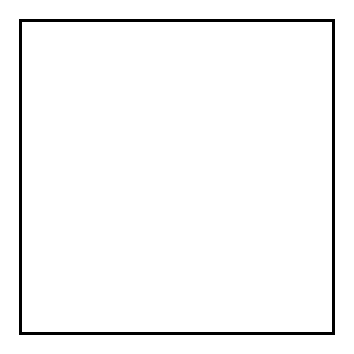
\includegraphics[totalheight=1in]{rosettebox}
	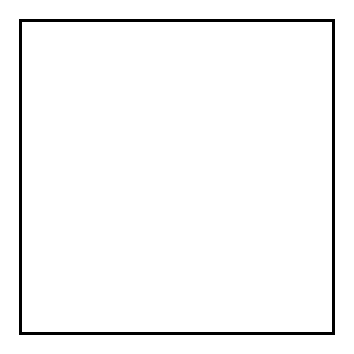
\includegraphics[angle=45,totalheight=1in]{rosettebox}
	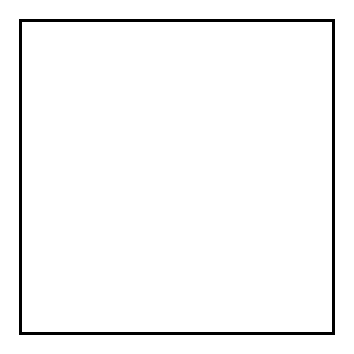
\includegraphics[angle=90,totalheight=1in]{rosettebox}
\end{center}
每一幅图像的结果是旋转后的BoundingBox 为1英寸高。
缩放功能改变的是BoundingBox 的大小,而不是实际看到图像的大小。


\subsection{旋转图形的对齐}\label{ssec:ralign}

\subsubsection{第一个例子}

当图形被旋转时,可能会出现不对齐的情况。例如:

\begin{lstlisting}
\begin{center}
   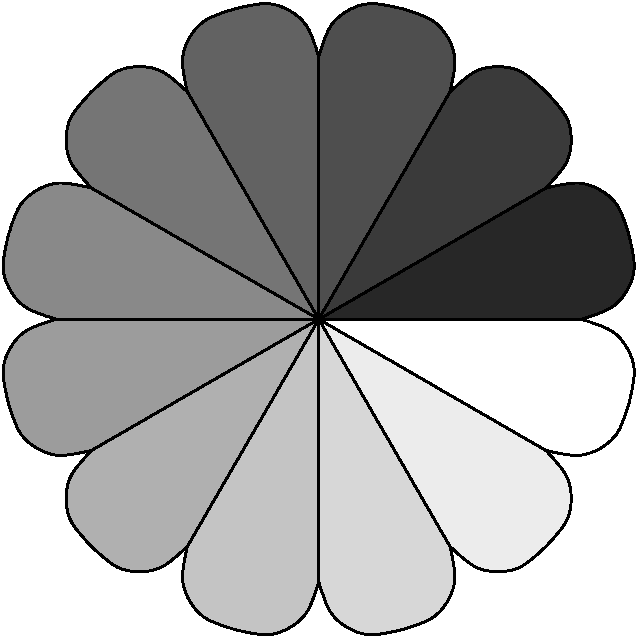
\includegraphics[totalheight=1in]{rosette}
   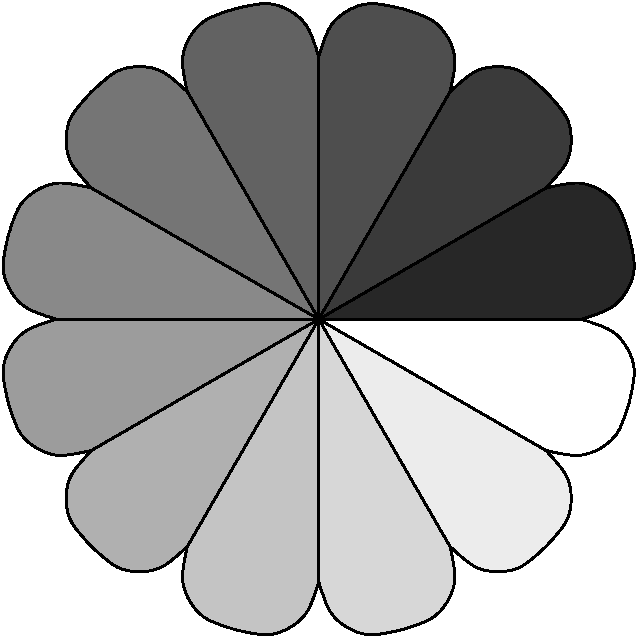
\includegraphics[totalheight=1in,angle=-45]{rosette}
   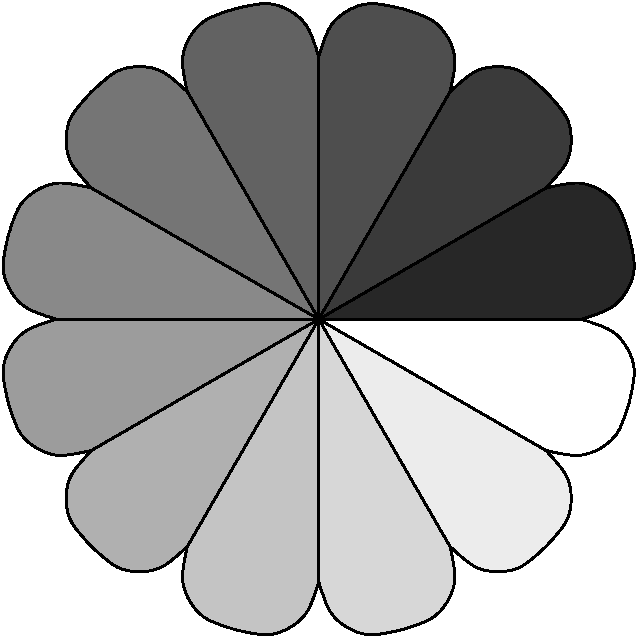
\includegraphics[totalheight=1in,angle=-90]{rosette}
\end{center}
\end{lstlisting}
得到

\begin{center}
   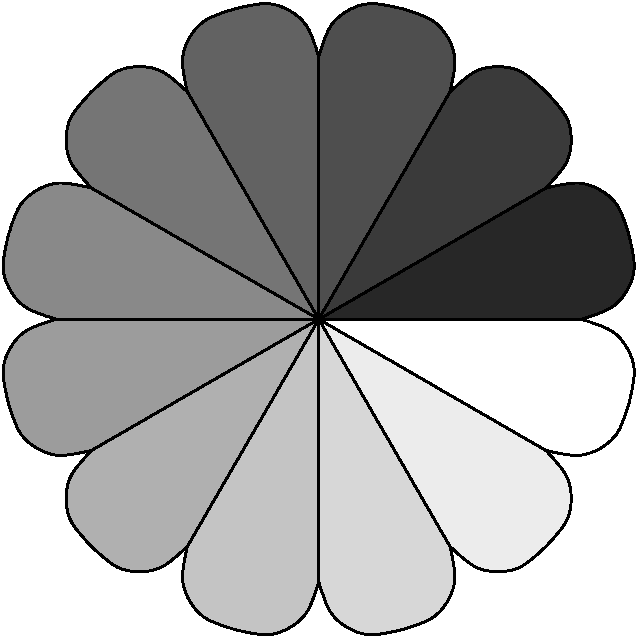
\includegraphics[totalheight=1in]{rosette}
   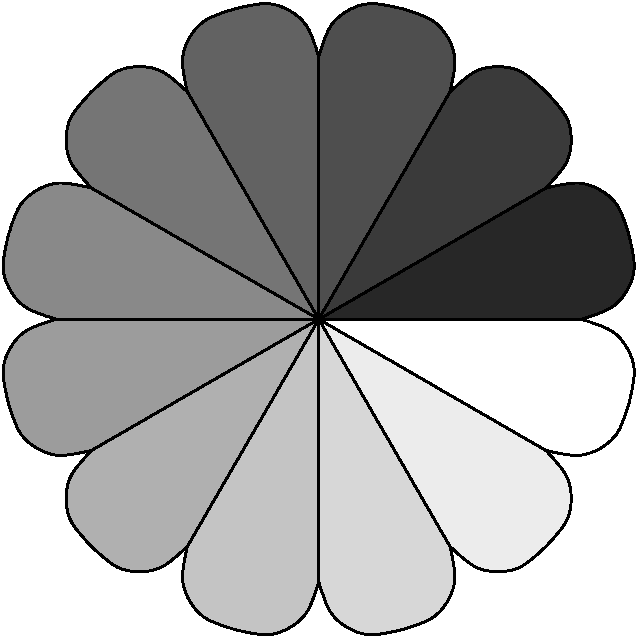
\includegraphics[totalheight=1in,angle=-45]{rosette}
   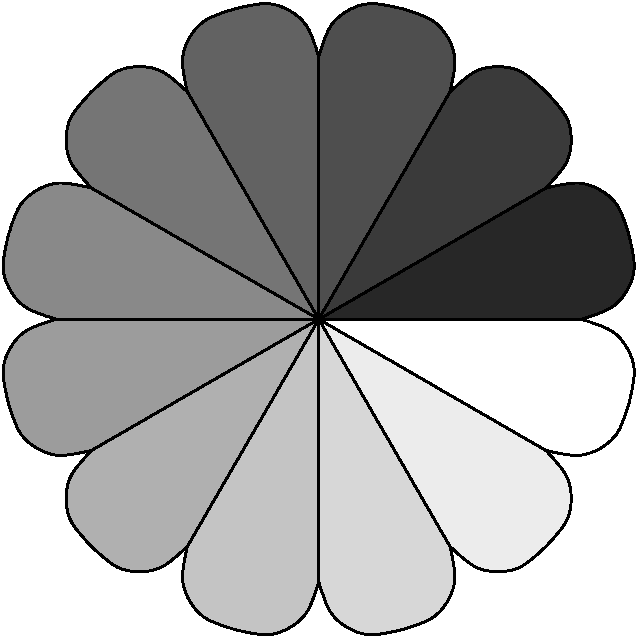
\includegraphics[totalheight=1in,angle=-90]{rosette}
\end{center}
当然,这种现象仍可用图形的~BoundingBox~来解释。

\begin{center}
   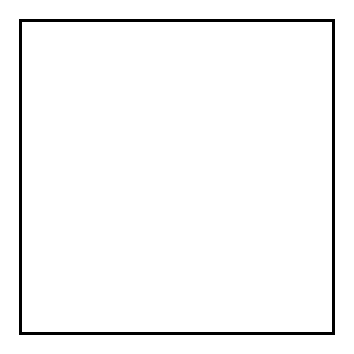
\includegraphics[totalheight=1in]{rosettebox}
   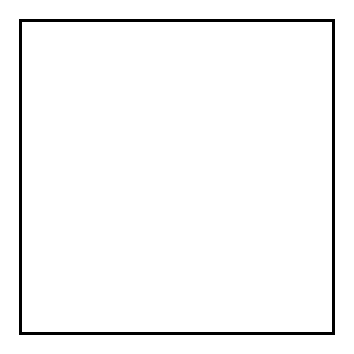
\includegraphics[totalheight=1in,angle=-45]{rosettebox}
   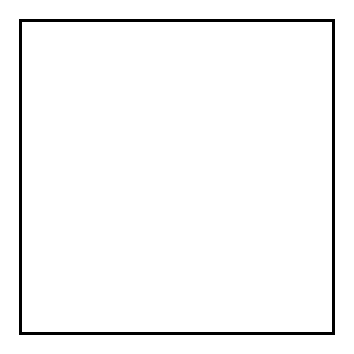
\includegraphics[totalheight=1in,angle=-90]{rosettebox}
\end{center}
在这种情况下,我们可以看到图形对象的参考点(左下角)是处于同一水平线上的。
如果希望是中间对齐,那么可以用 \cmd{includegraphics} 的 \opt{origin} 选项。
\begin{lstlisting}
\begin{center}
   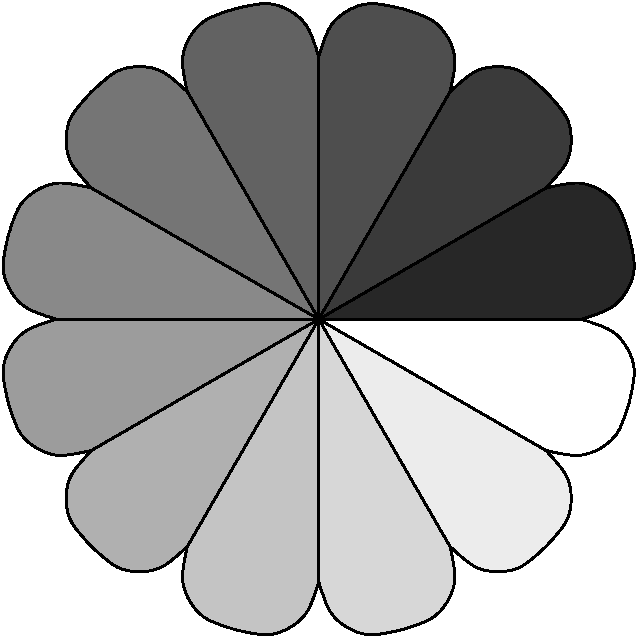
\includegraphics[totalheight=1in]{rosette}
   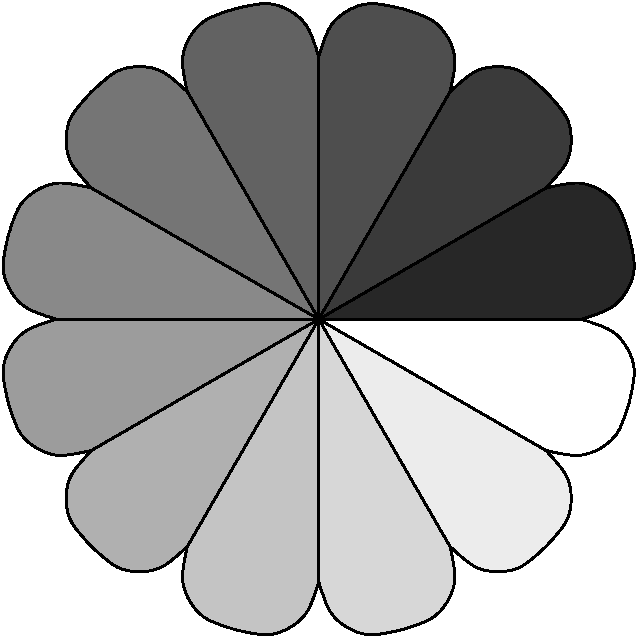
\includegraphics[totalheight=1in,origin=c,angle=-45]{rosette}
   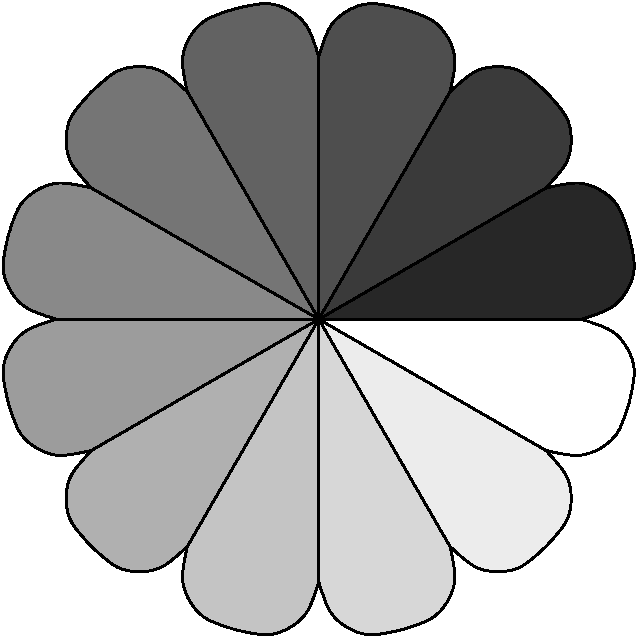
\includegraphics[totalheight=1in,origin=c,angle=-90]{rosette}
\end{center}
\end{lstlisting}
这次所有图形都是中间对齐的。

\begin{center}
   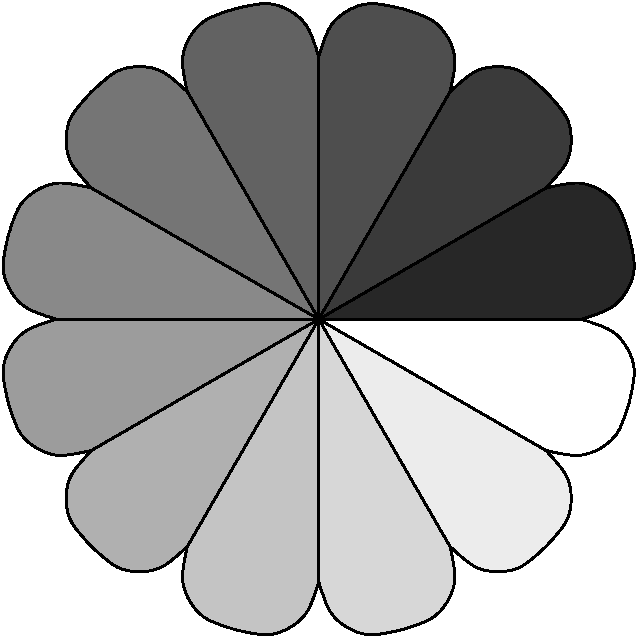
\includegraphics[totalheight=1in]{rosette}
   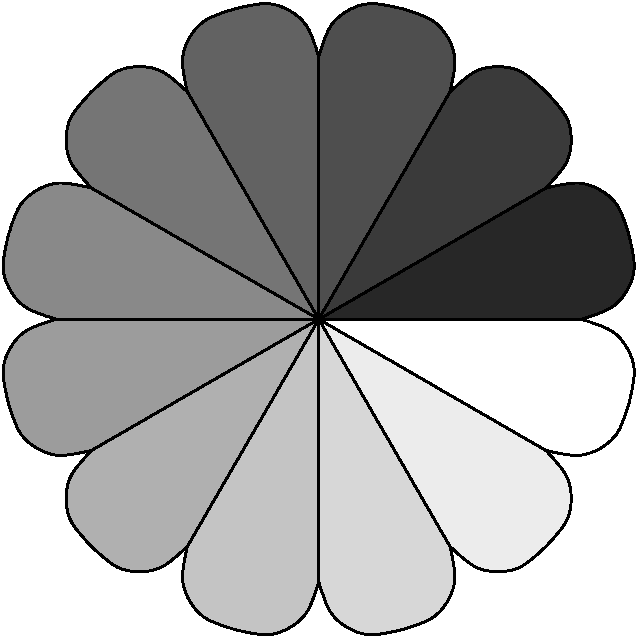
\includegraphics[totalheight=1in,origin=c,angle=-45]{rosette}
   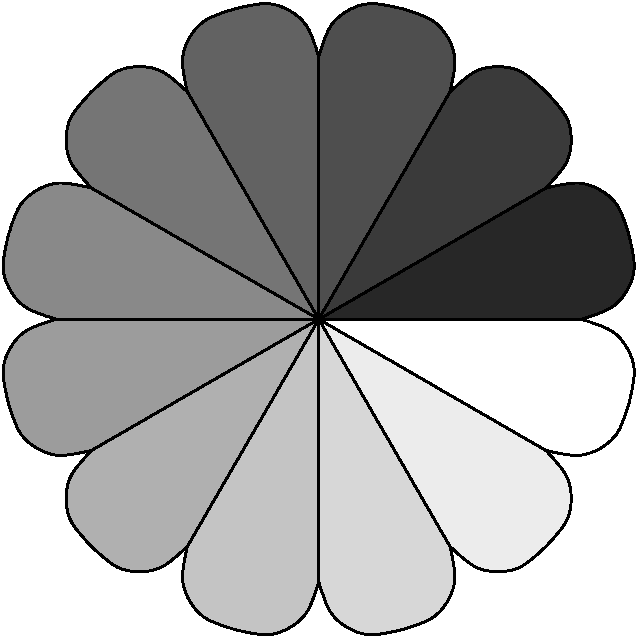
\includegraphics[totalheight=1in,origin=c,angle=-90]{rosette}
\end{center}

\subsubsection{第二个例子}
同样地,下面的命令
\begin{lstlisting}
\begin{center}
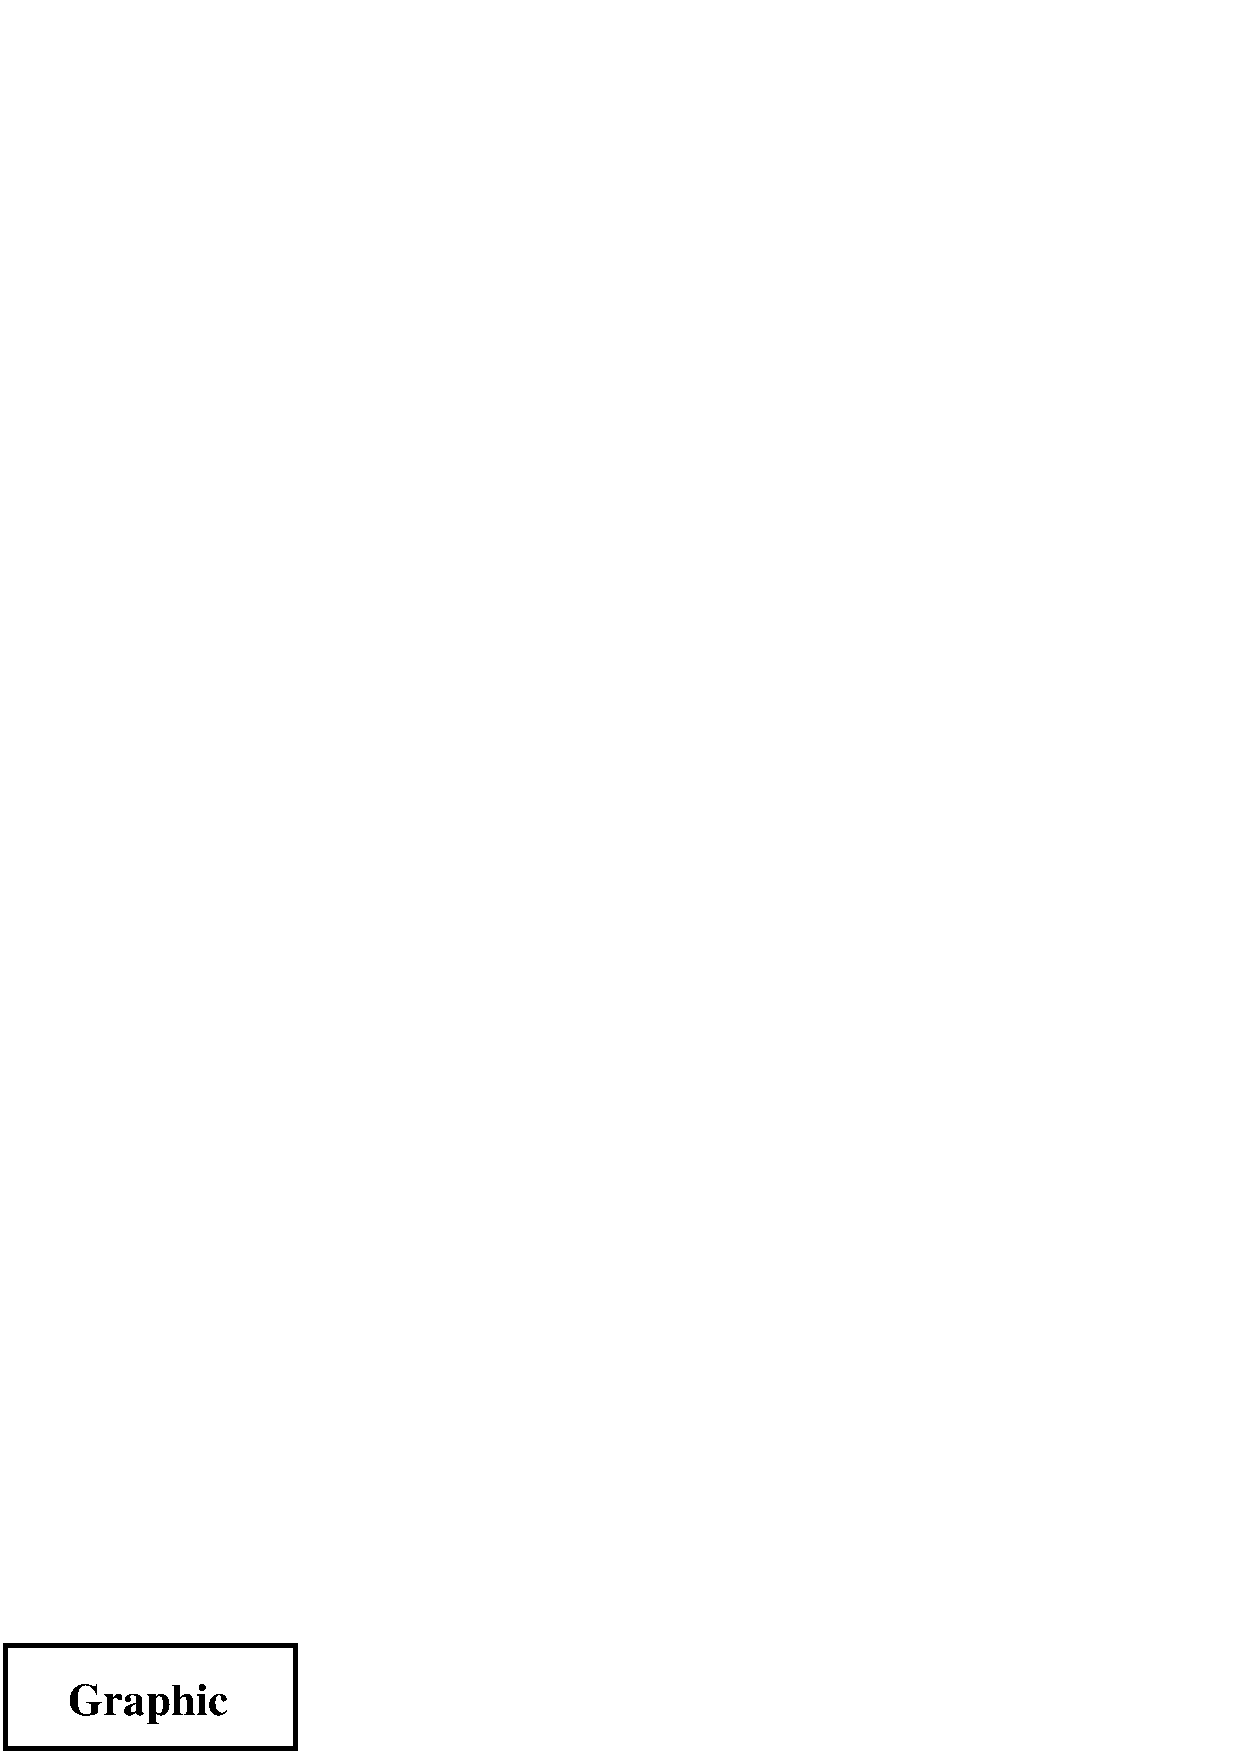
\includegraphics[width=1in]{graphic}
\hspace{1in}
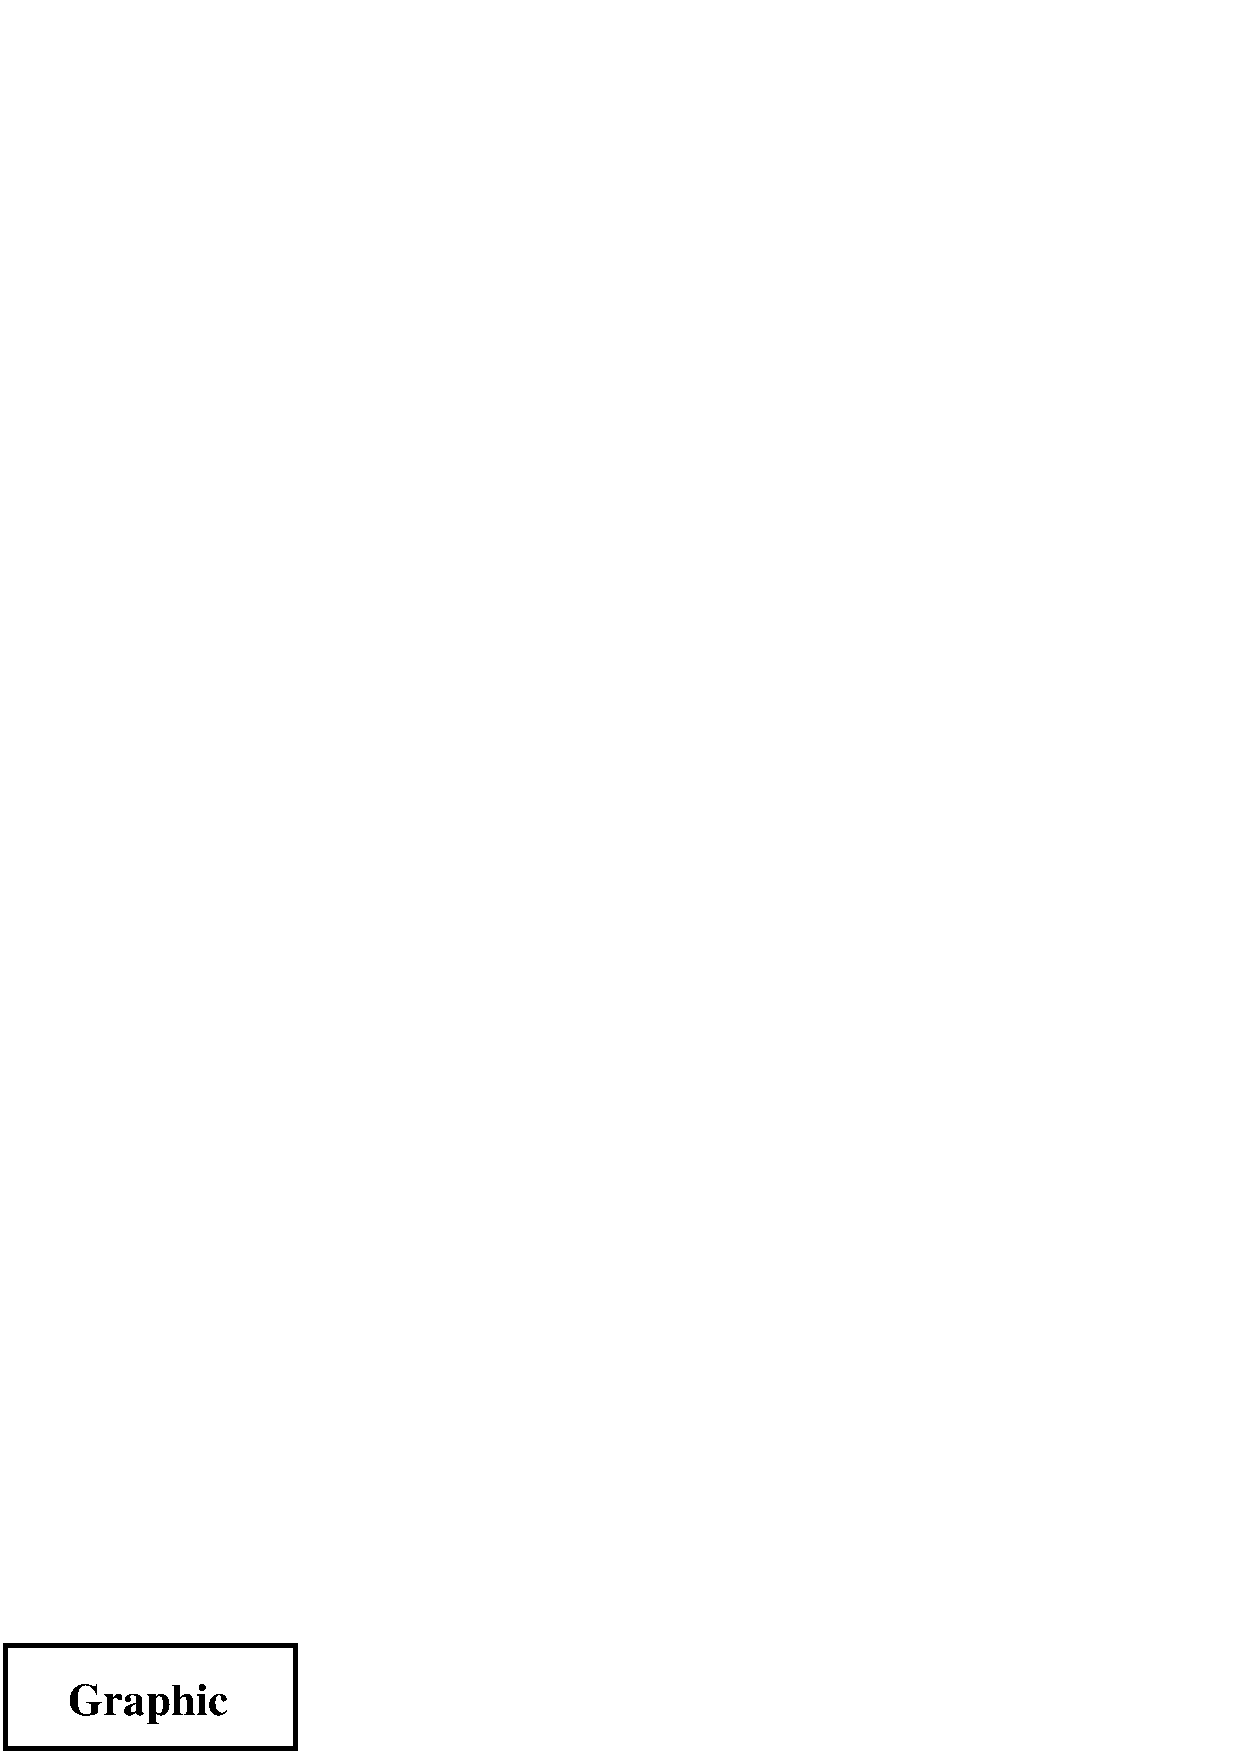
\includegraphics[width=1in,angle=-90]{graphic}
\end{center}
\end{lstlisting}
将右边的图形绕它的左下角旋转,得到如下结果:
\begin{center}
	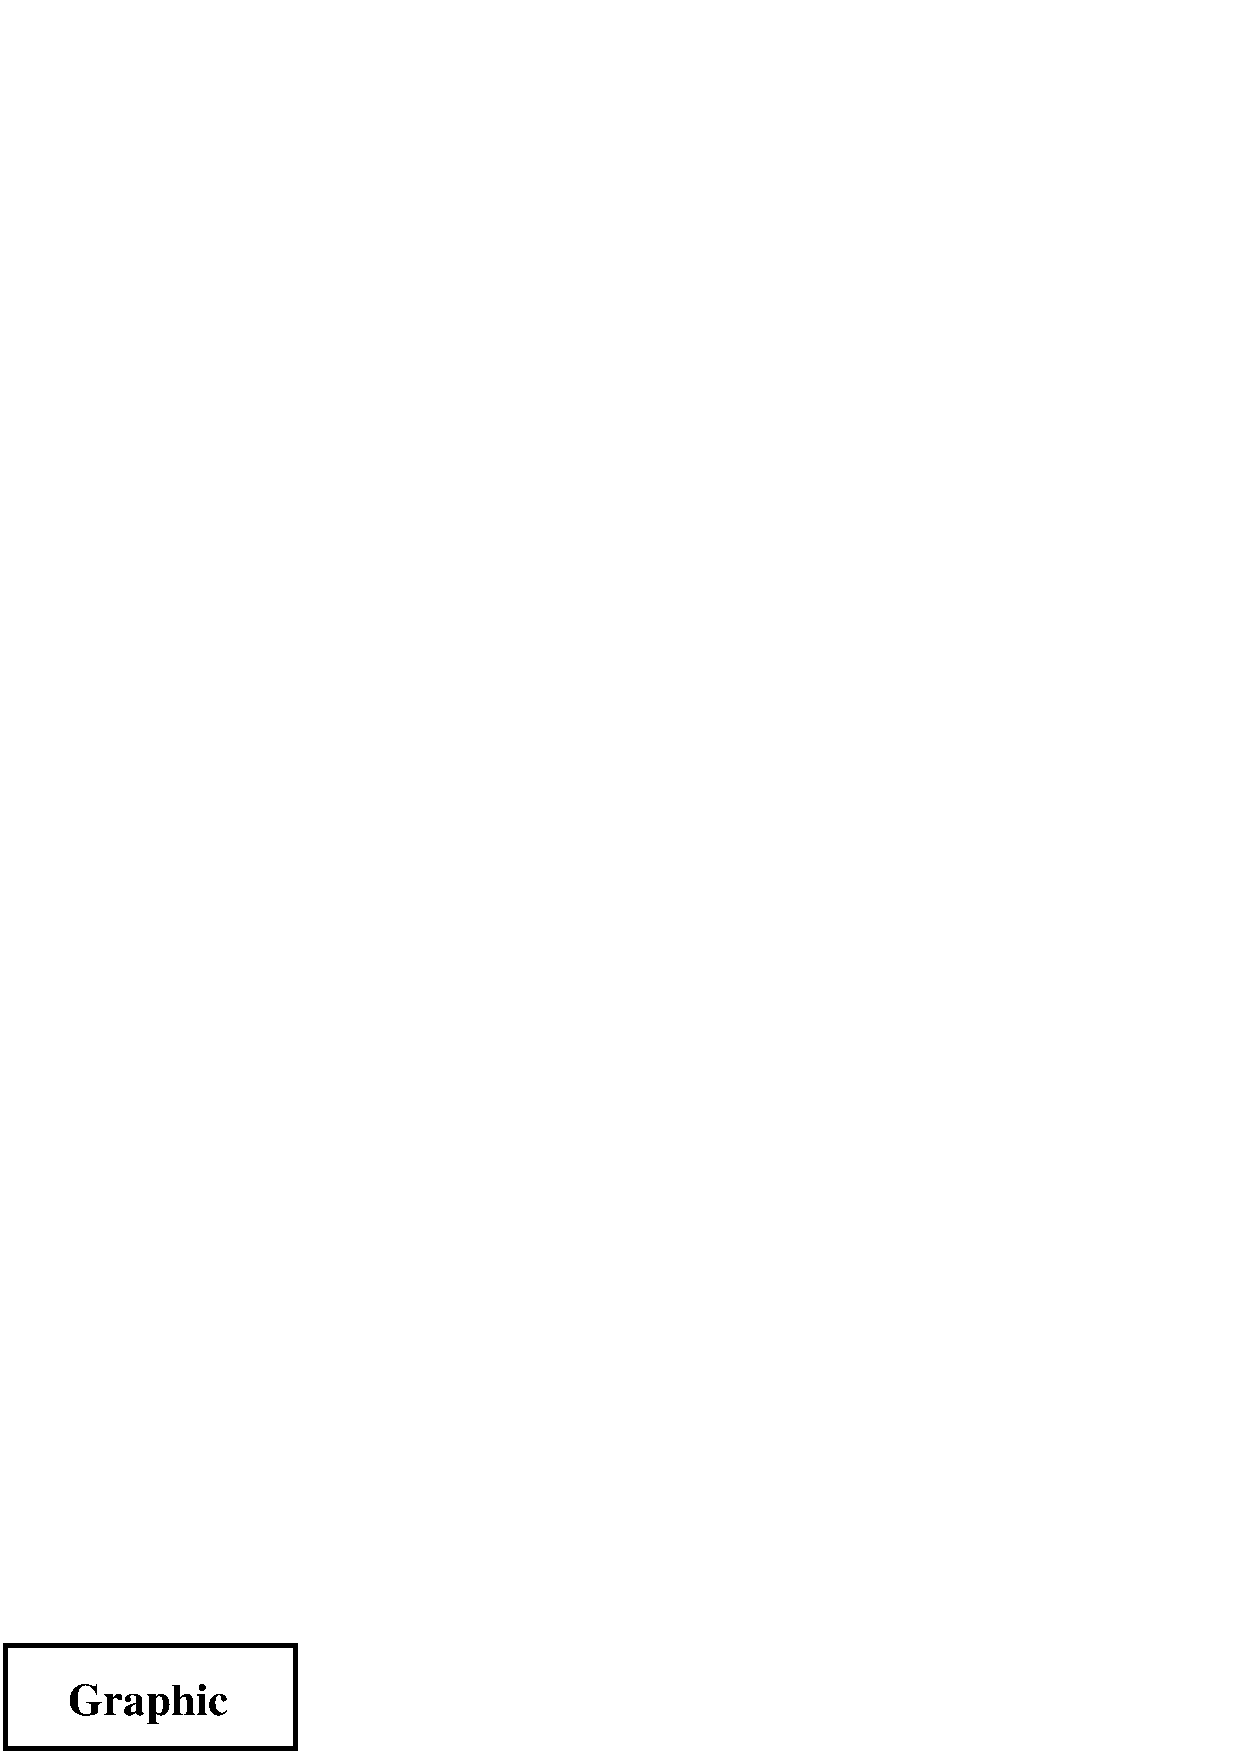
\includegraphics[width=1in]{graphic}
	\hspace{1in}
	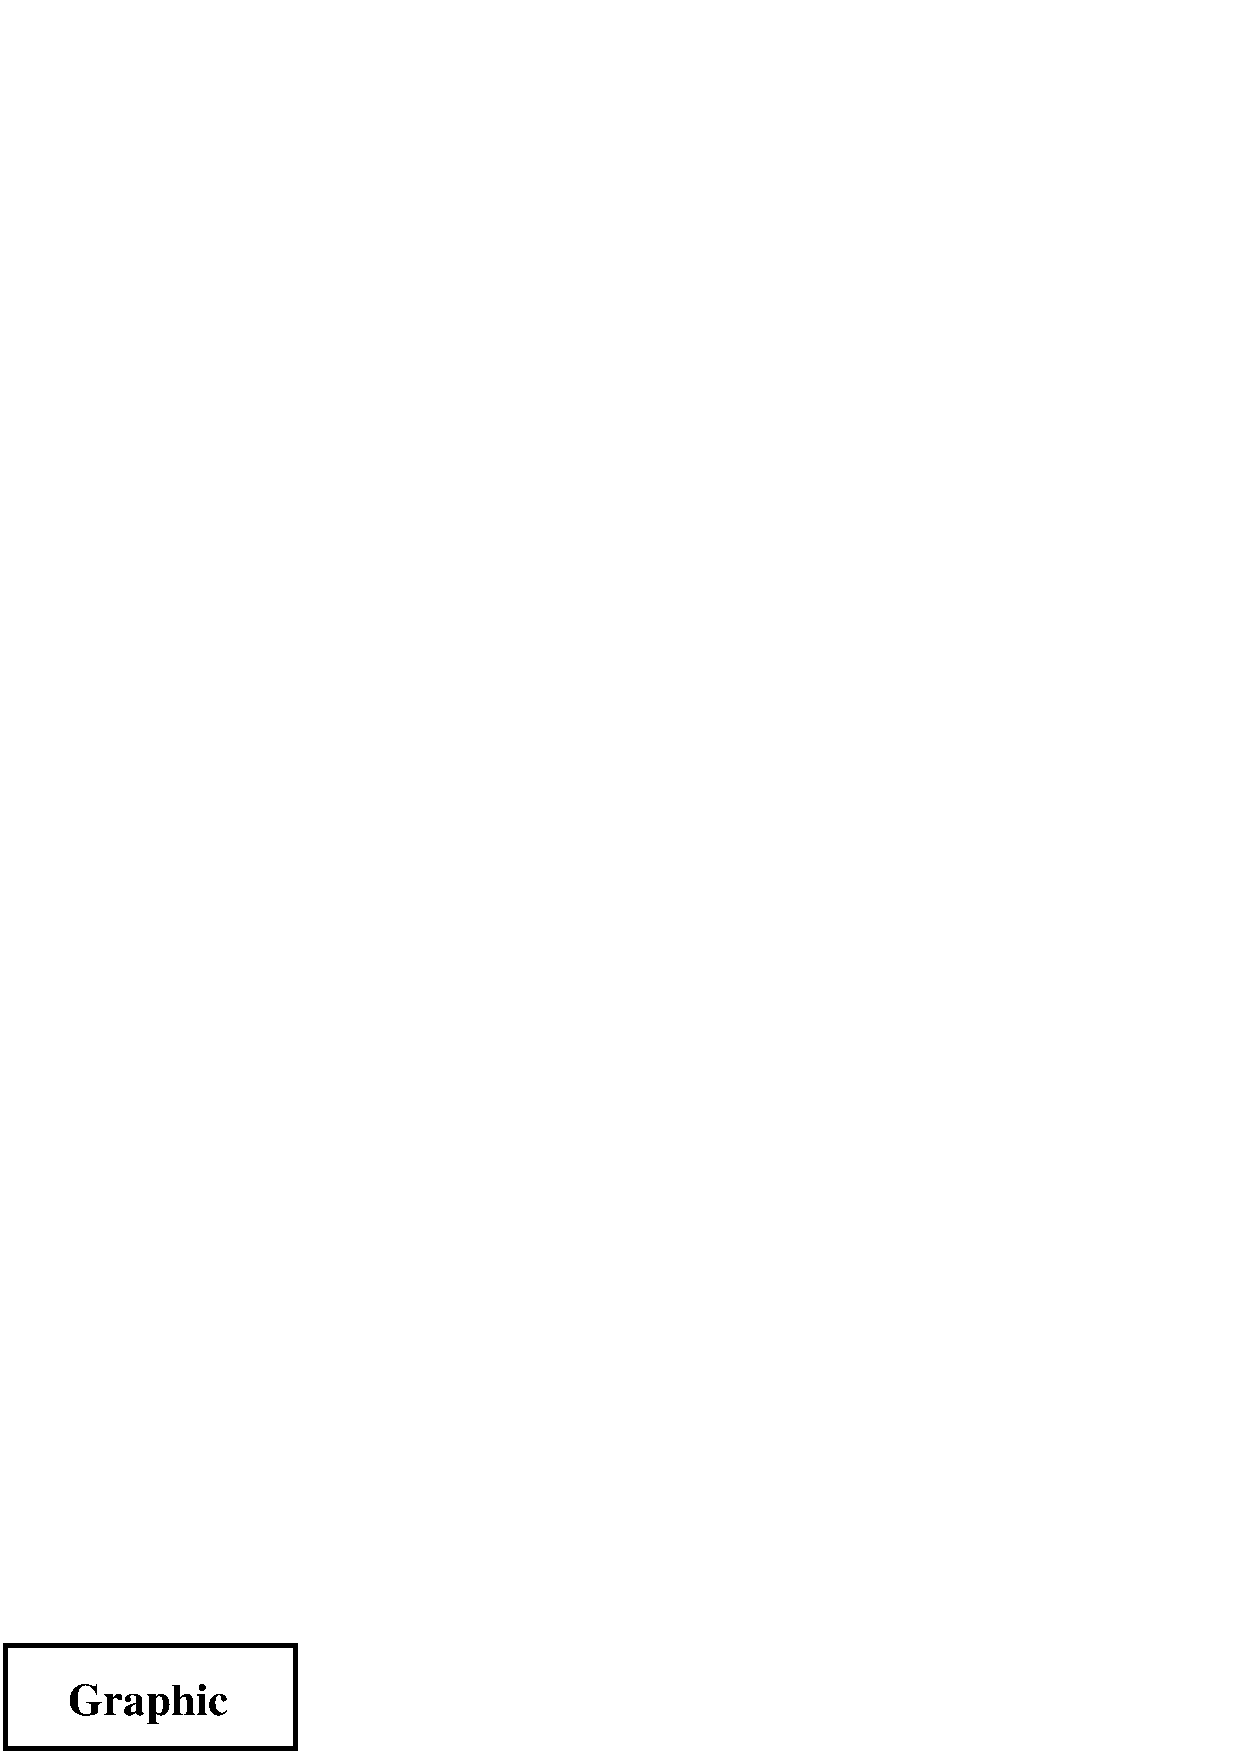
\includegraphics[width=1in,angle=-90]{graphic}
\end{center}

要想使图形的底部对齐,使用下面的命令:
\begin{lstlisting}
\begin{center}
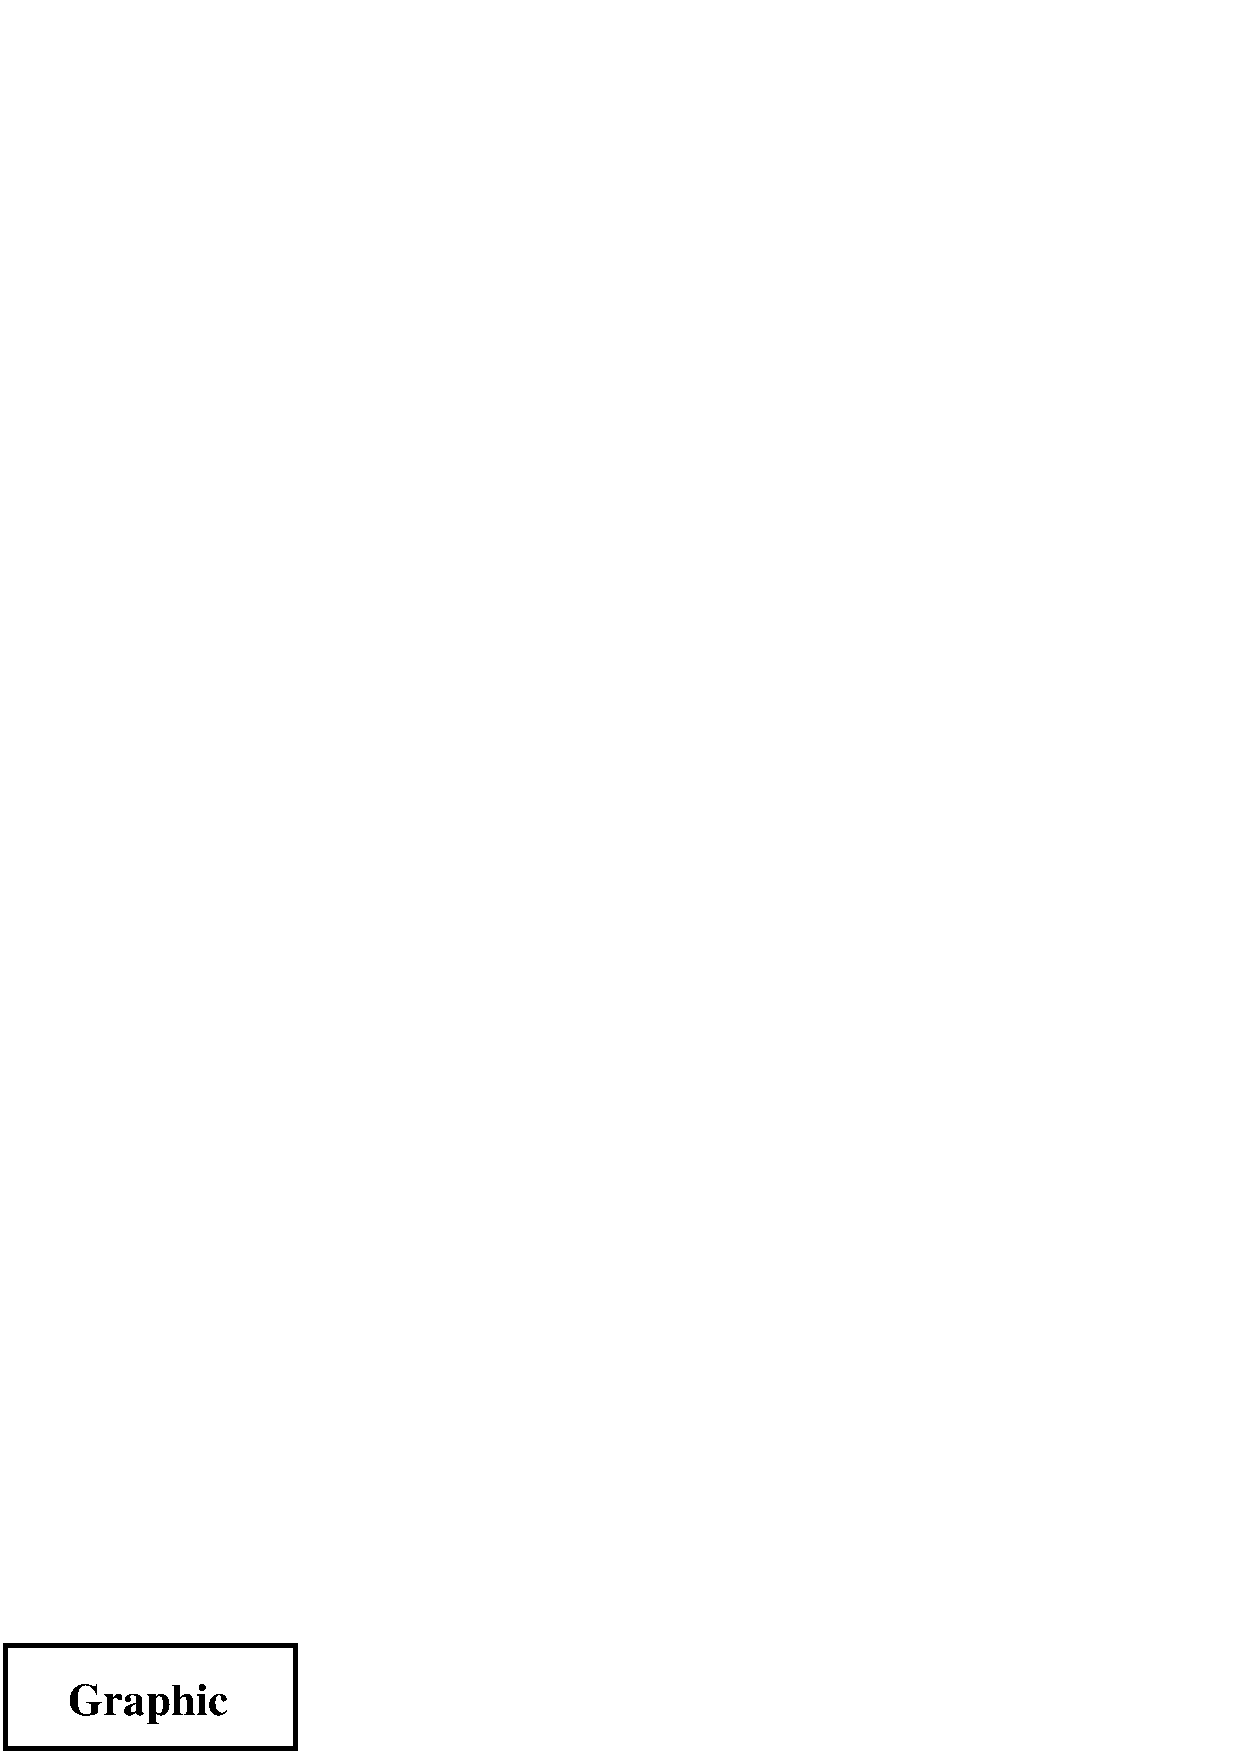
\includegraphics[width=1in]{graphic}
\hspace{1in}
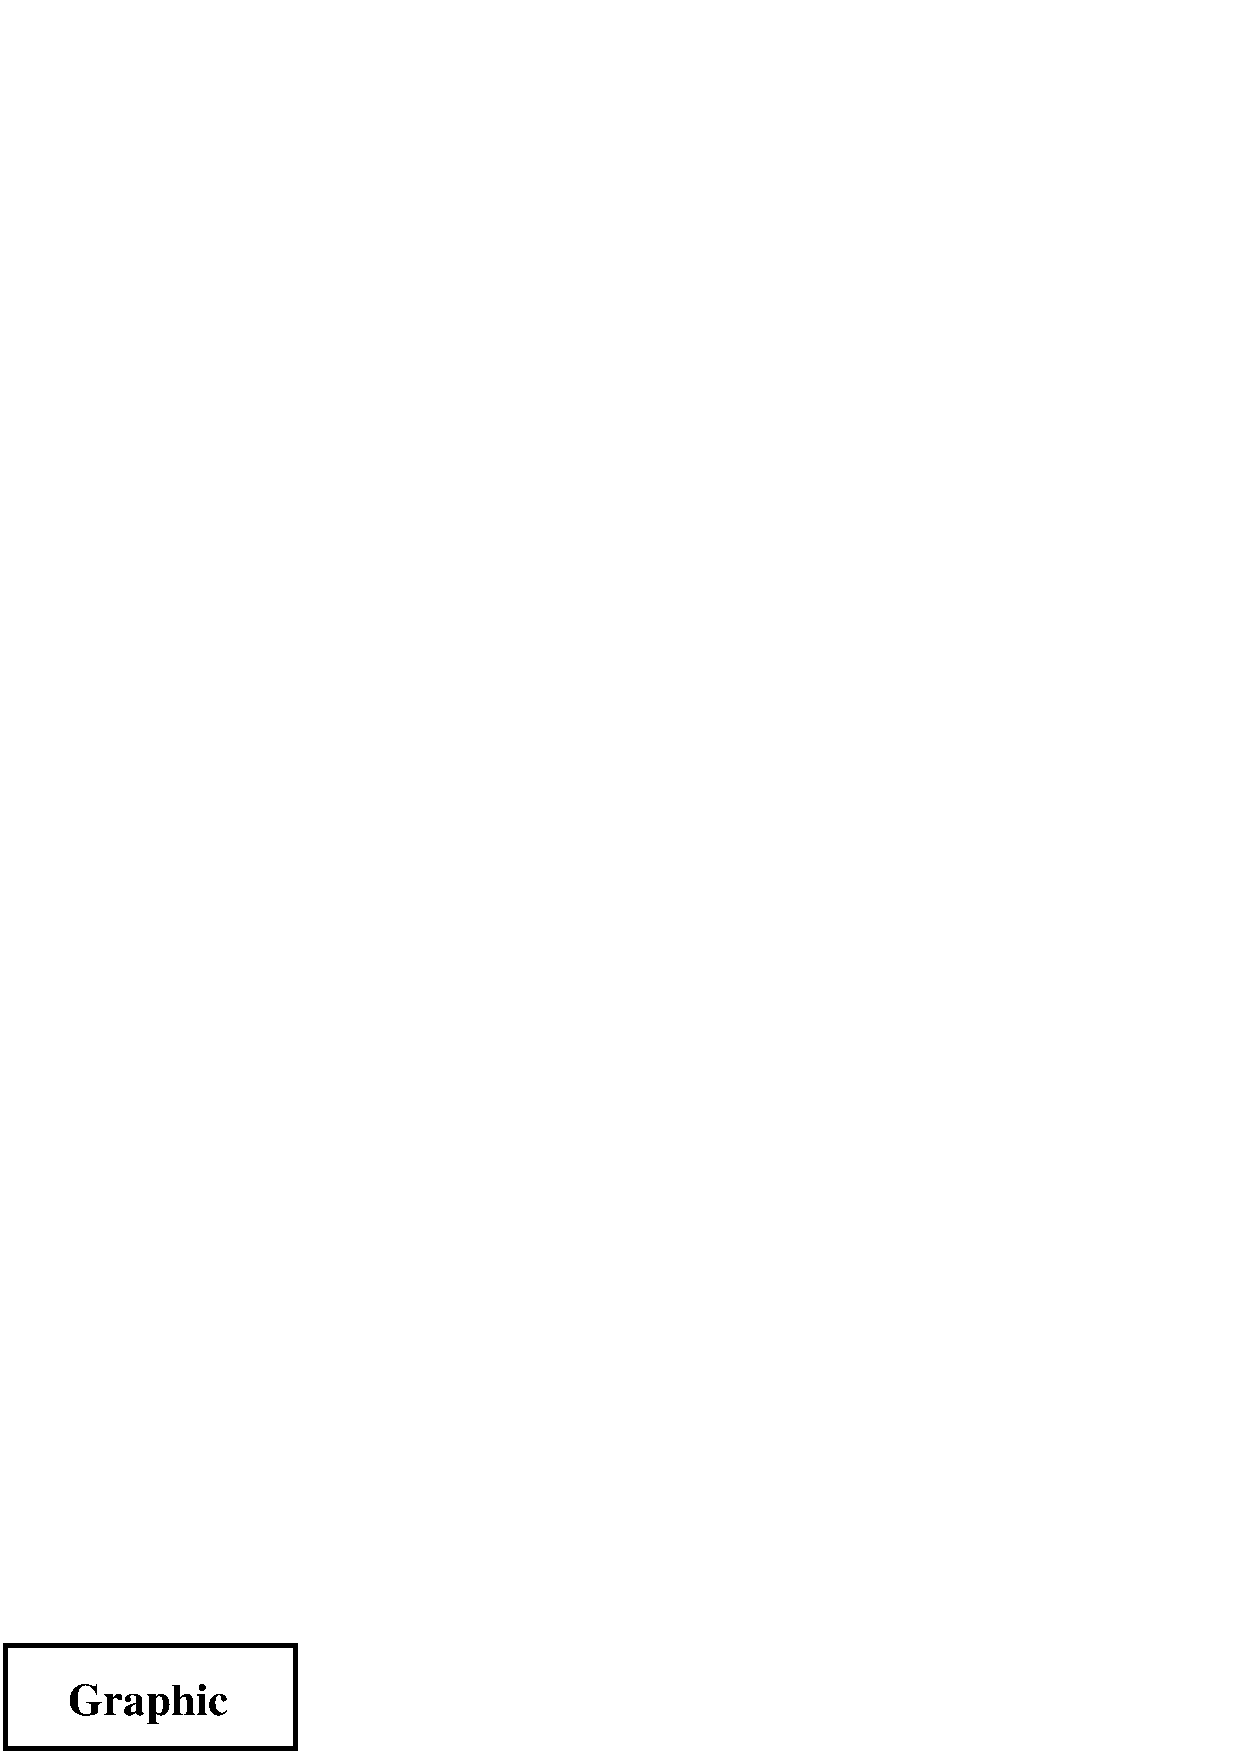
\includegraphics[width=1in,origin=br,angle=-90]{graphic}
\end{center}
\end{lstlisting}
上述命令让右边的图形绕它的右下角旋转,得到如下结果:
\begin{center}
	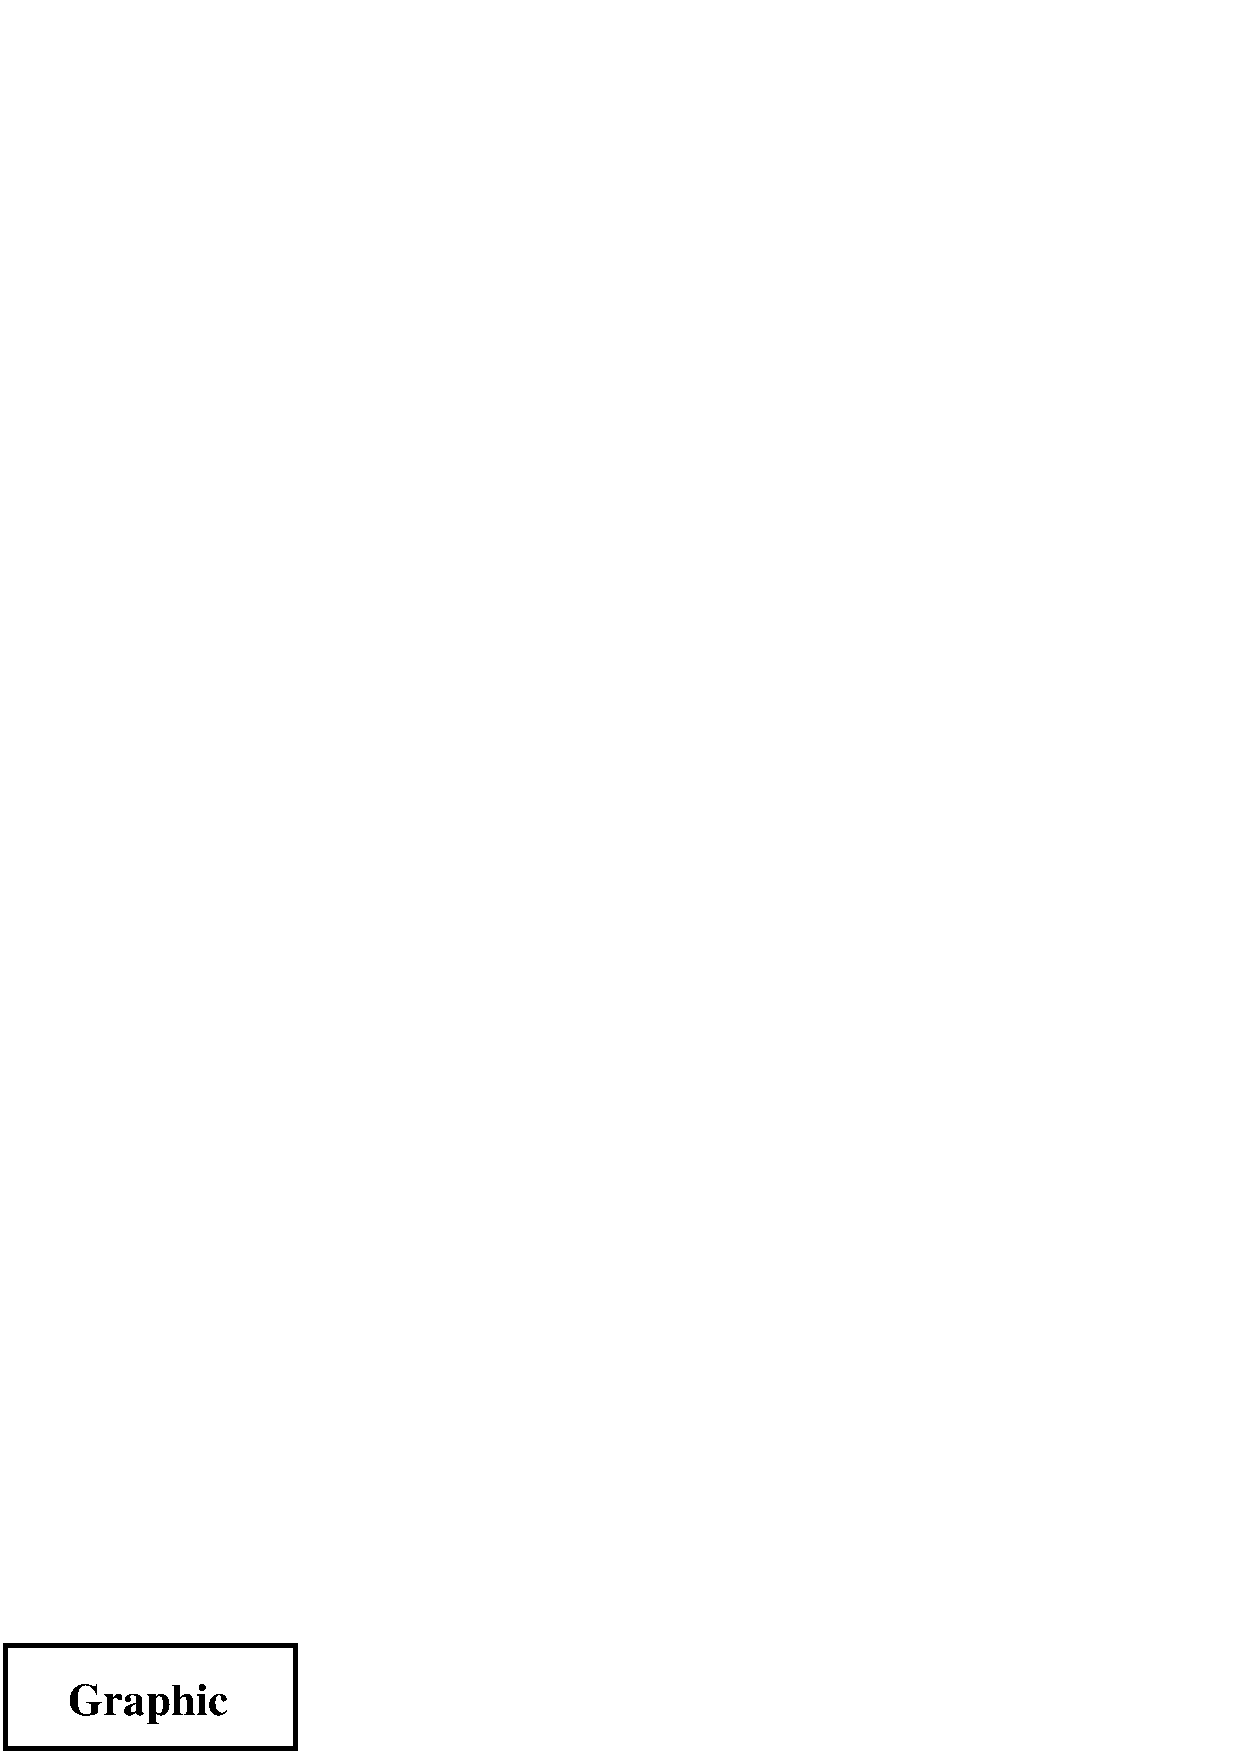
\includegraphics[width=1in]{graphic}
	\hspace{1in}
	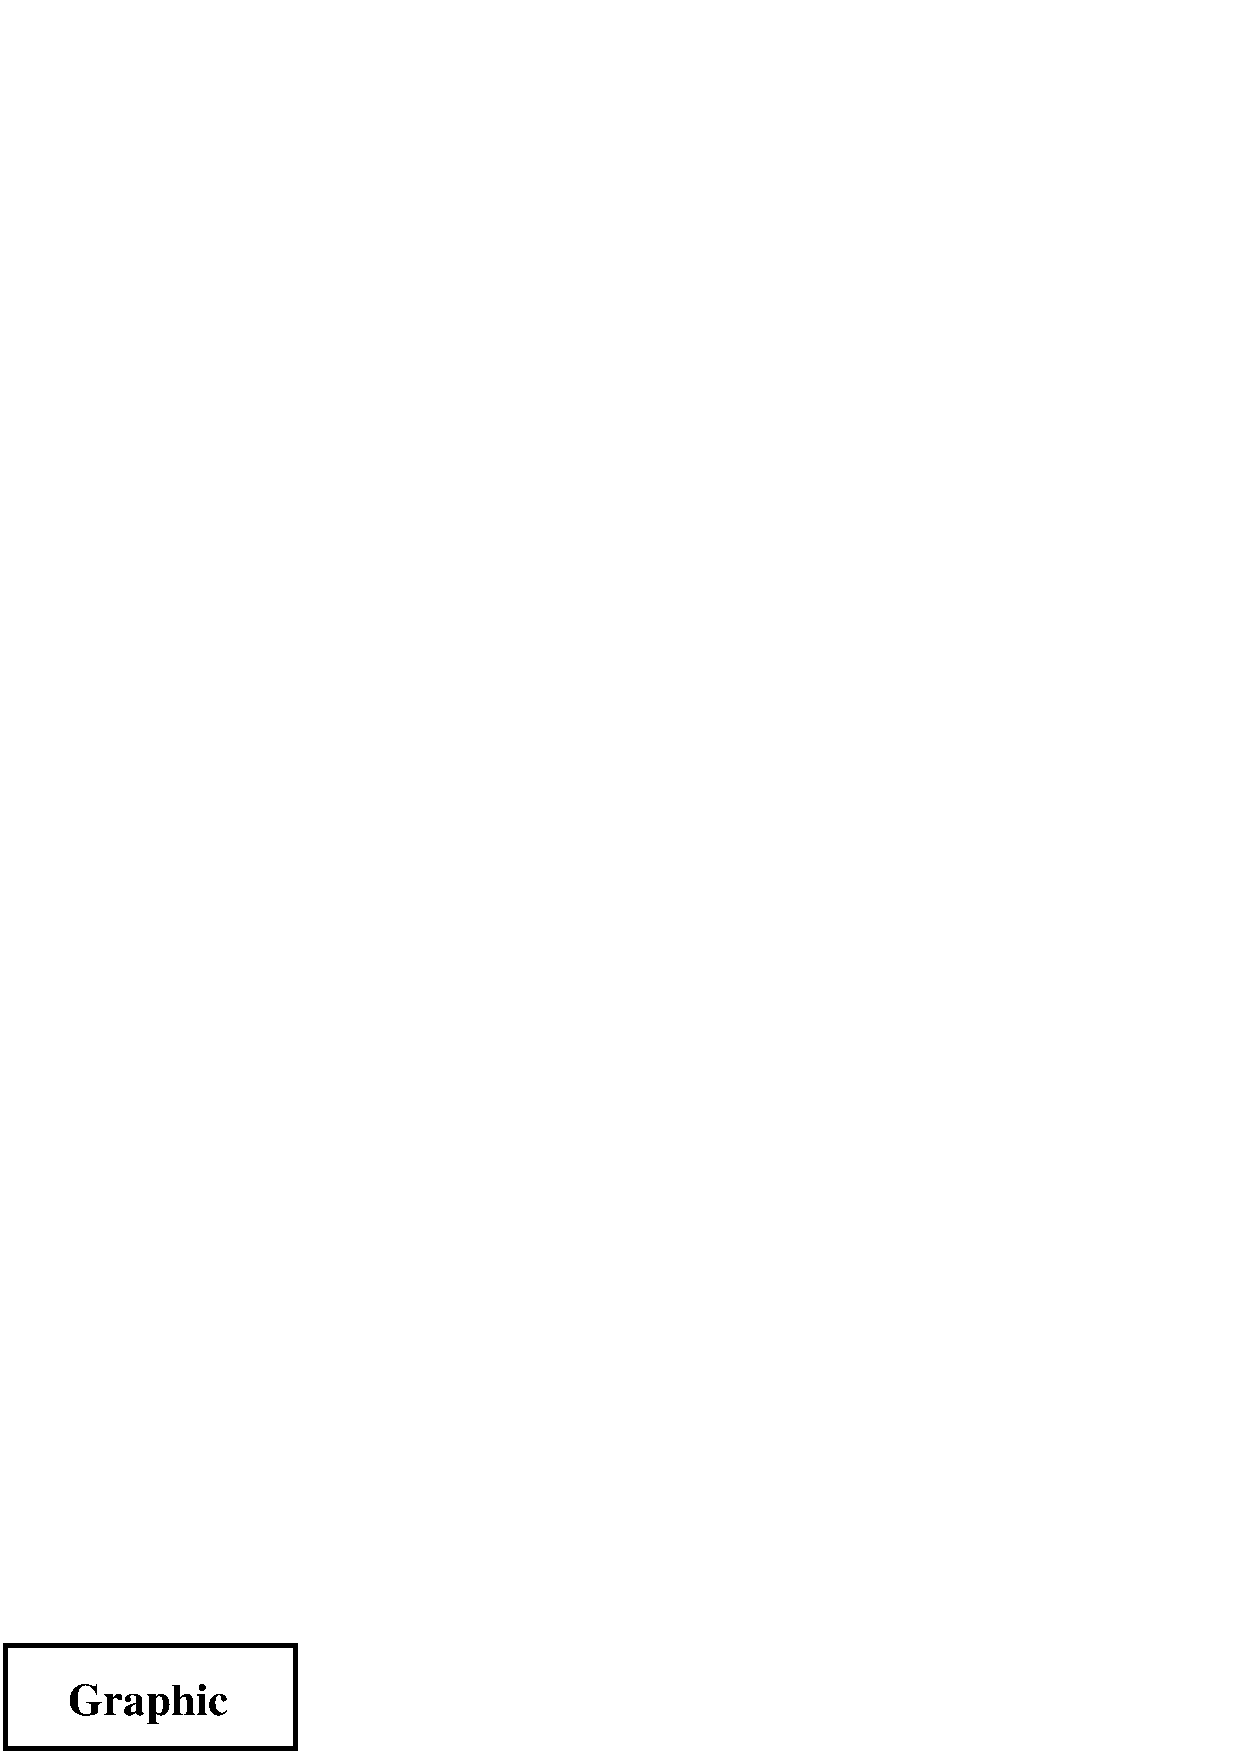
\includegraphics[width=1in,origin=br,angle=-90]{graphic}
\end{center}

\subsection{小页环境的垂直对齐}\label{ssec:minivalign}

将图形放置于 \envi{minipage} 小页环境中是经常遇到的情况下,
而且也十分实用(见第~\ref{sec:sidebyside}~节)。
当小页并列时, \LaTeX{} 会将它们的参考点垂直对齐地排列。
缺省地,小页的参考点是它的左边界的中点。
可用一个可选参数项来改变小页的参考点的位置。
\begin{description}
	\item[\opt{[b]}] 使小页的参考点与小页底行的参考点对齐。
	\item[\opt{[t]}] 使小页的参考点与小页顶行的参考点对齐。
\end{description}

注意选项 \opt{[b]} 不会将参考点置于小页的底部
(除非其底行的参考点在它的底部),
同样地,选项 \opt{[t]}~不会将参考点置于小页的顶部
(除非其顶行的参考点在它的顶部)。

当小页中只有一行时, \opt{[b]} 和 \opt{[t]} 选项得到的结果是一样的。例如:
\begin{lstlisting}
\begin{center}
\begin{minipage}[b]{.25\linewidth}
\centering
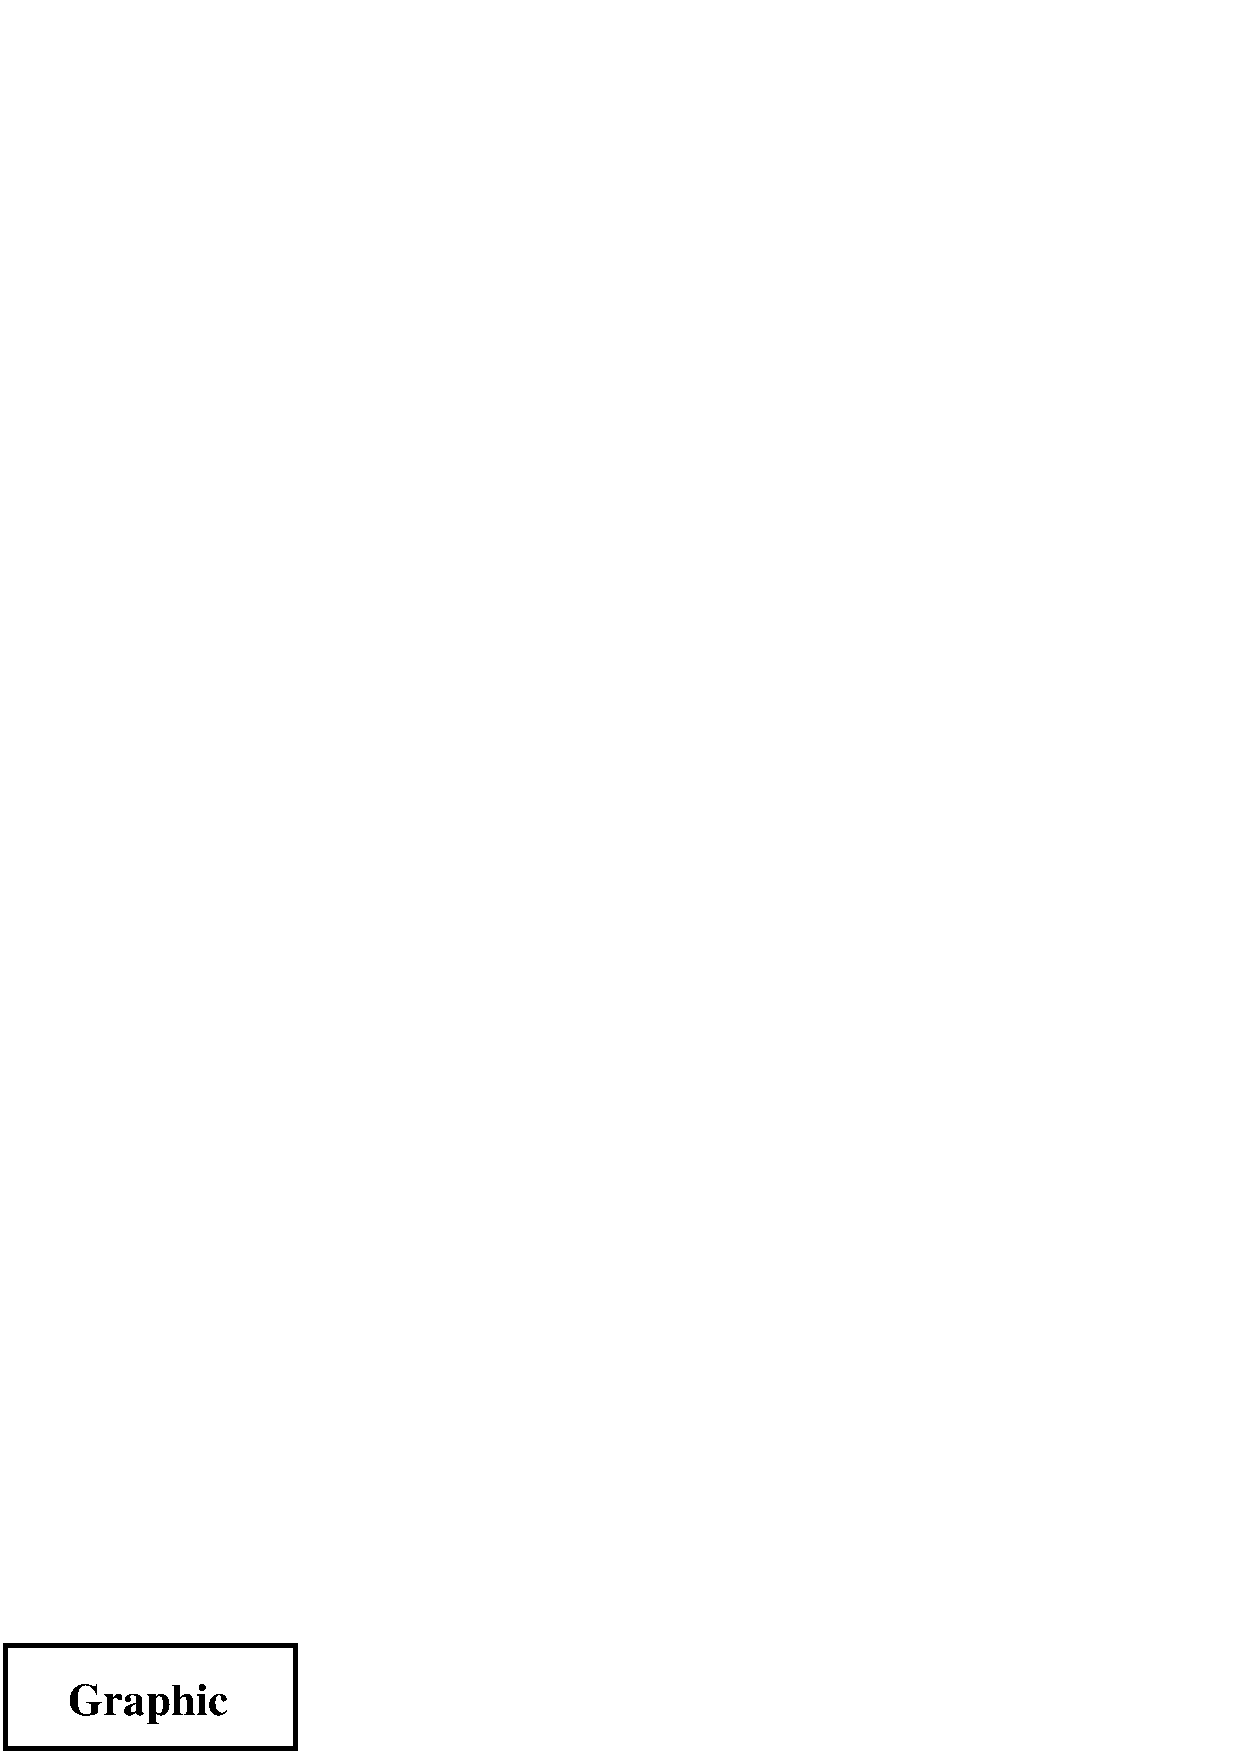
\includegraphics[width=1in]{graphic}
\end{minipage}%
\begin{minipage}[b]{.25\linewidth}
\centering
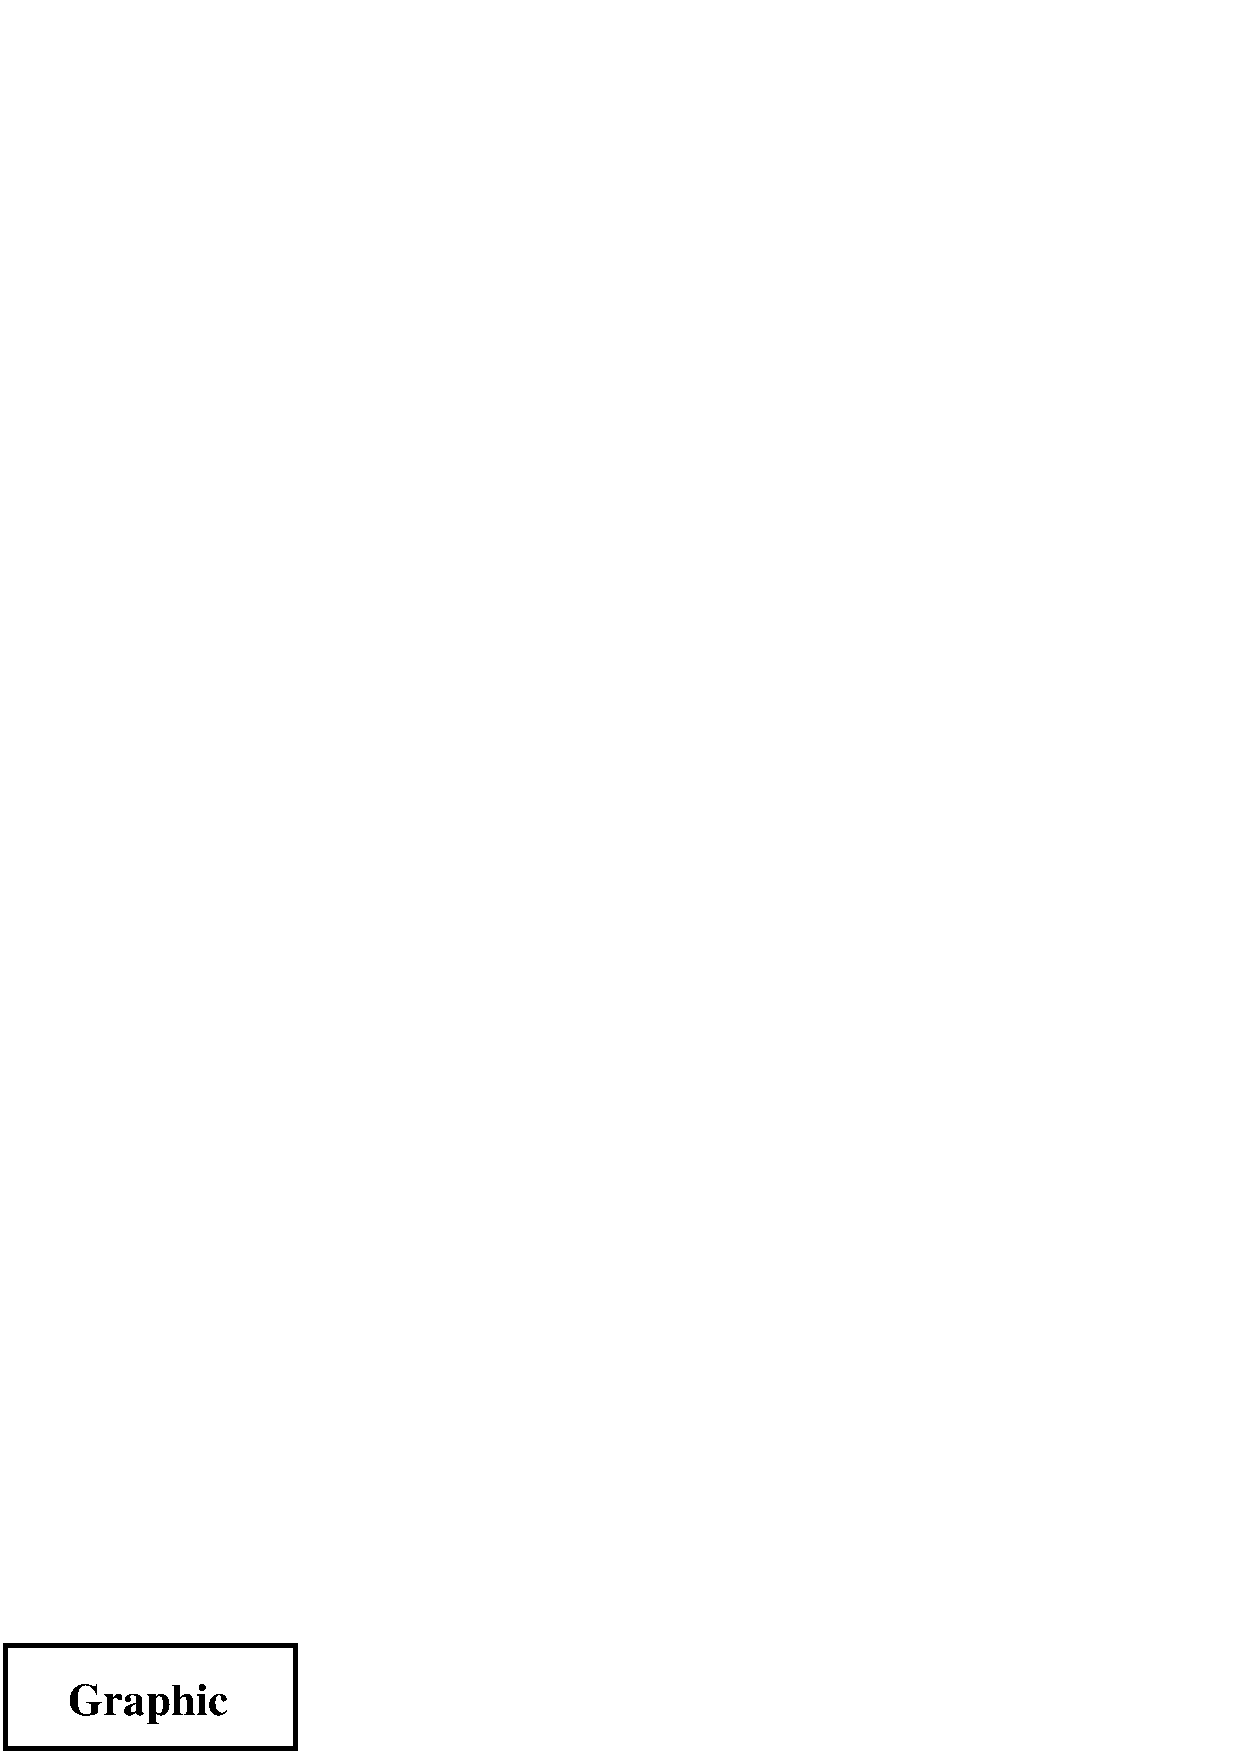
\includegraphics[width=1in,angle=-45]{graphic}
\end{minipage}
\end{center}
\end{lstlisting}
和
\begin{lstlisting}
\begin{center}
\begin{minipage}[t]{.25\linewidth}
\centering
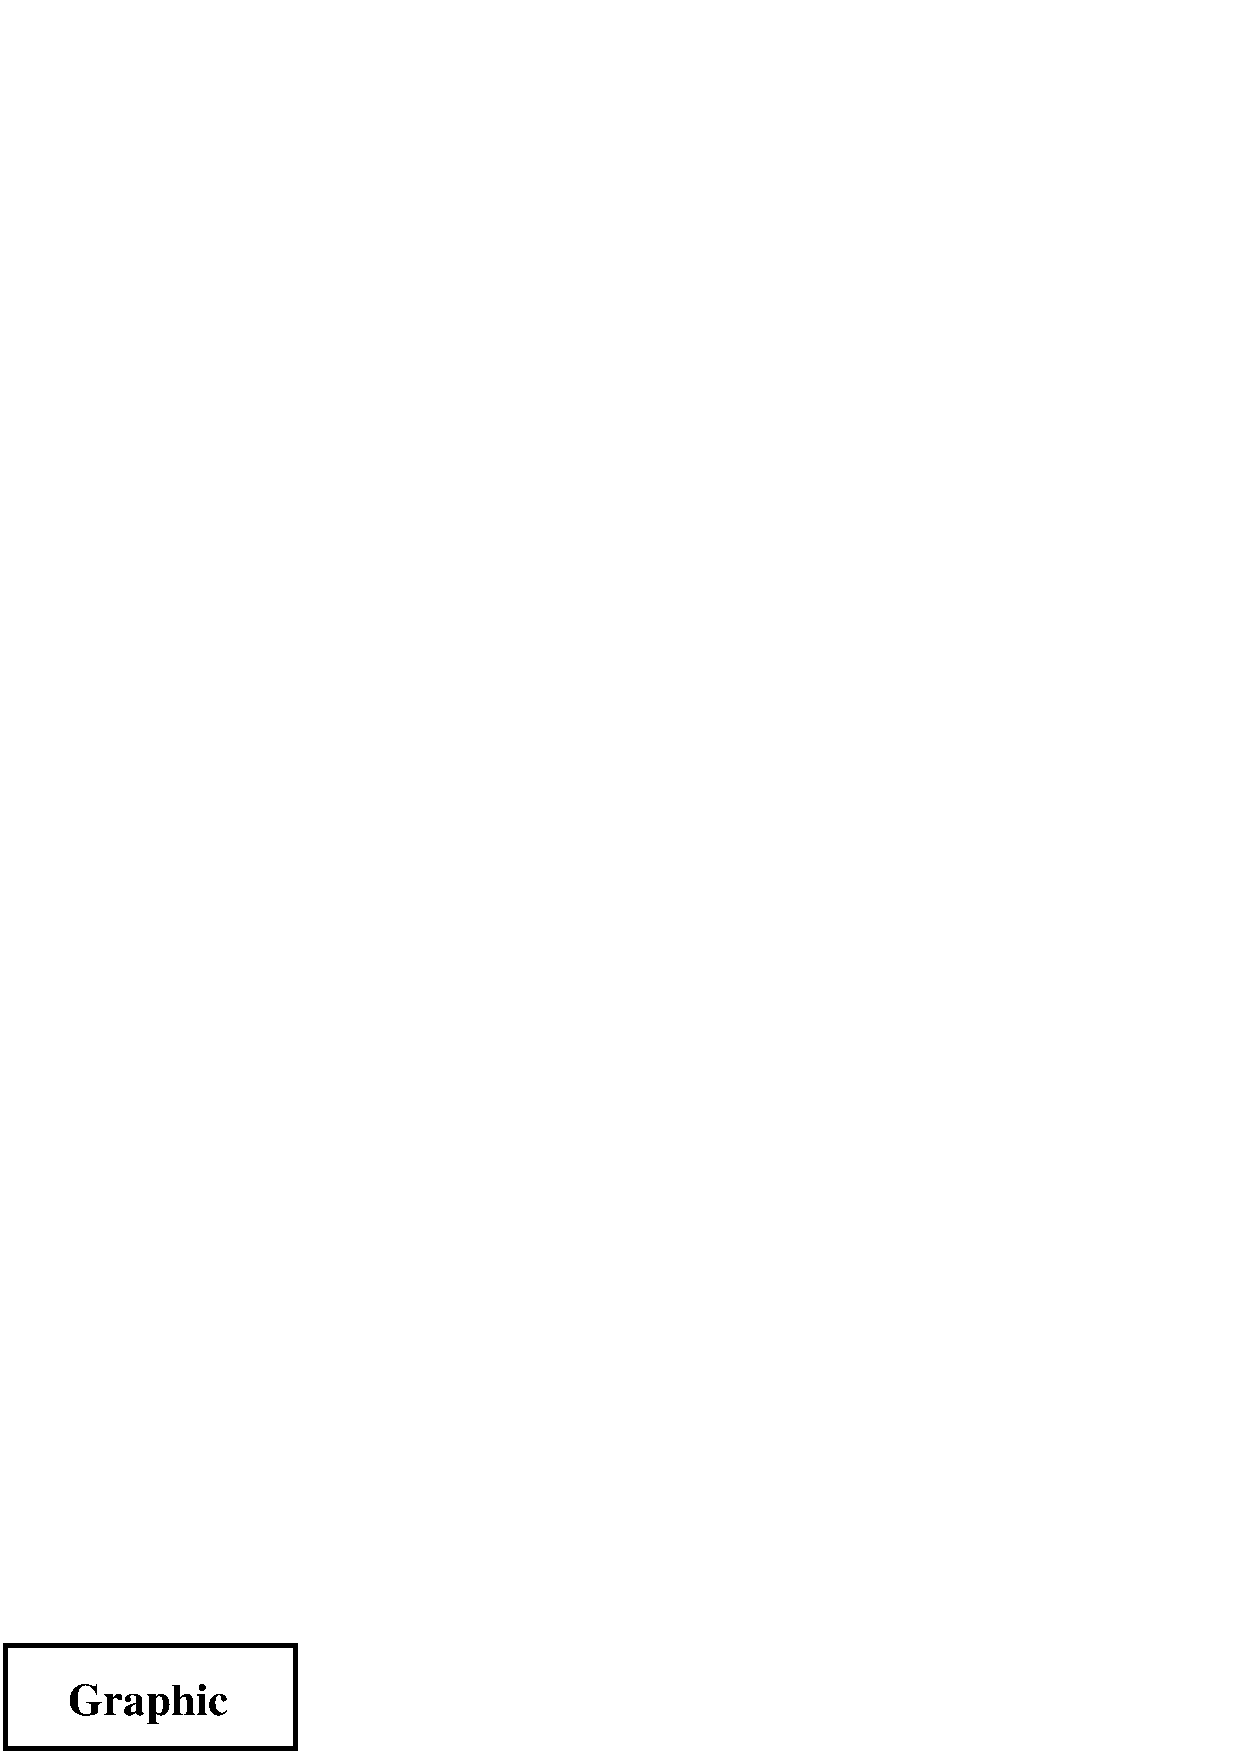
\includegraphics[width=1in]{graphic}
\end{minipage}%
\begin{minipage}[t]{.25\linewidth}
\centering
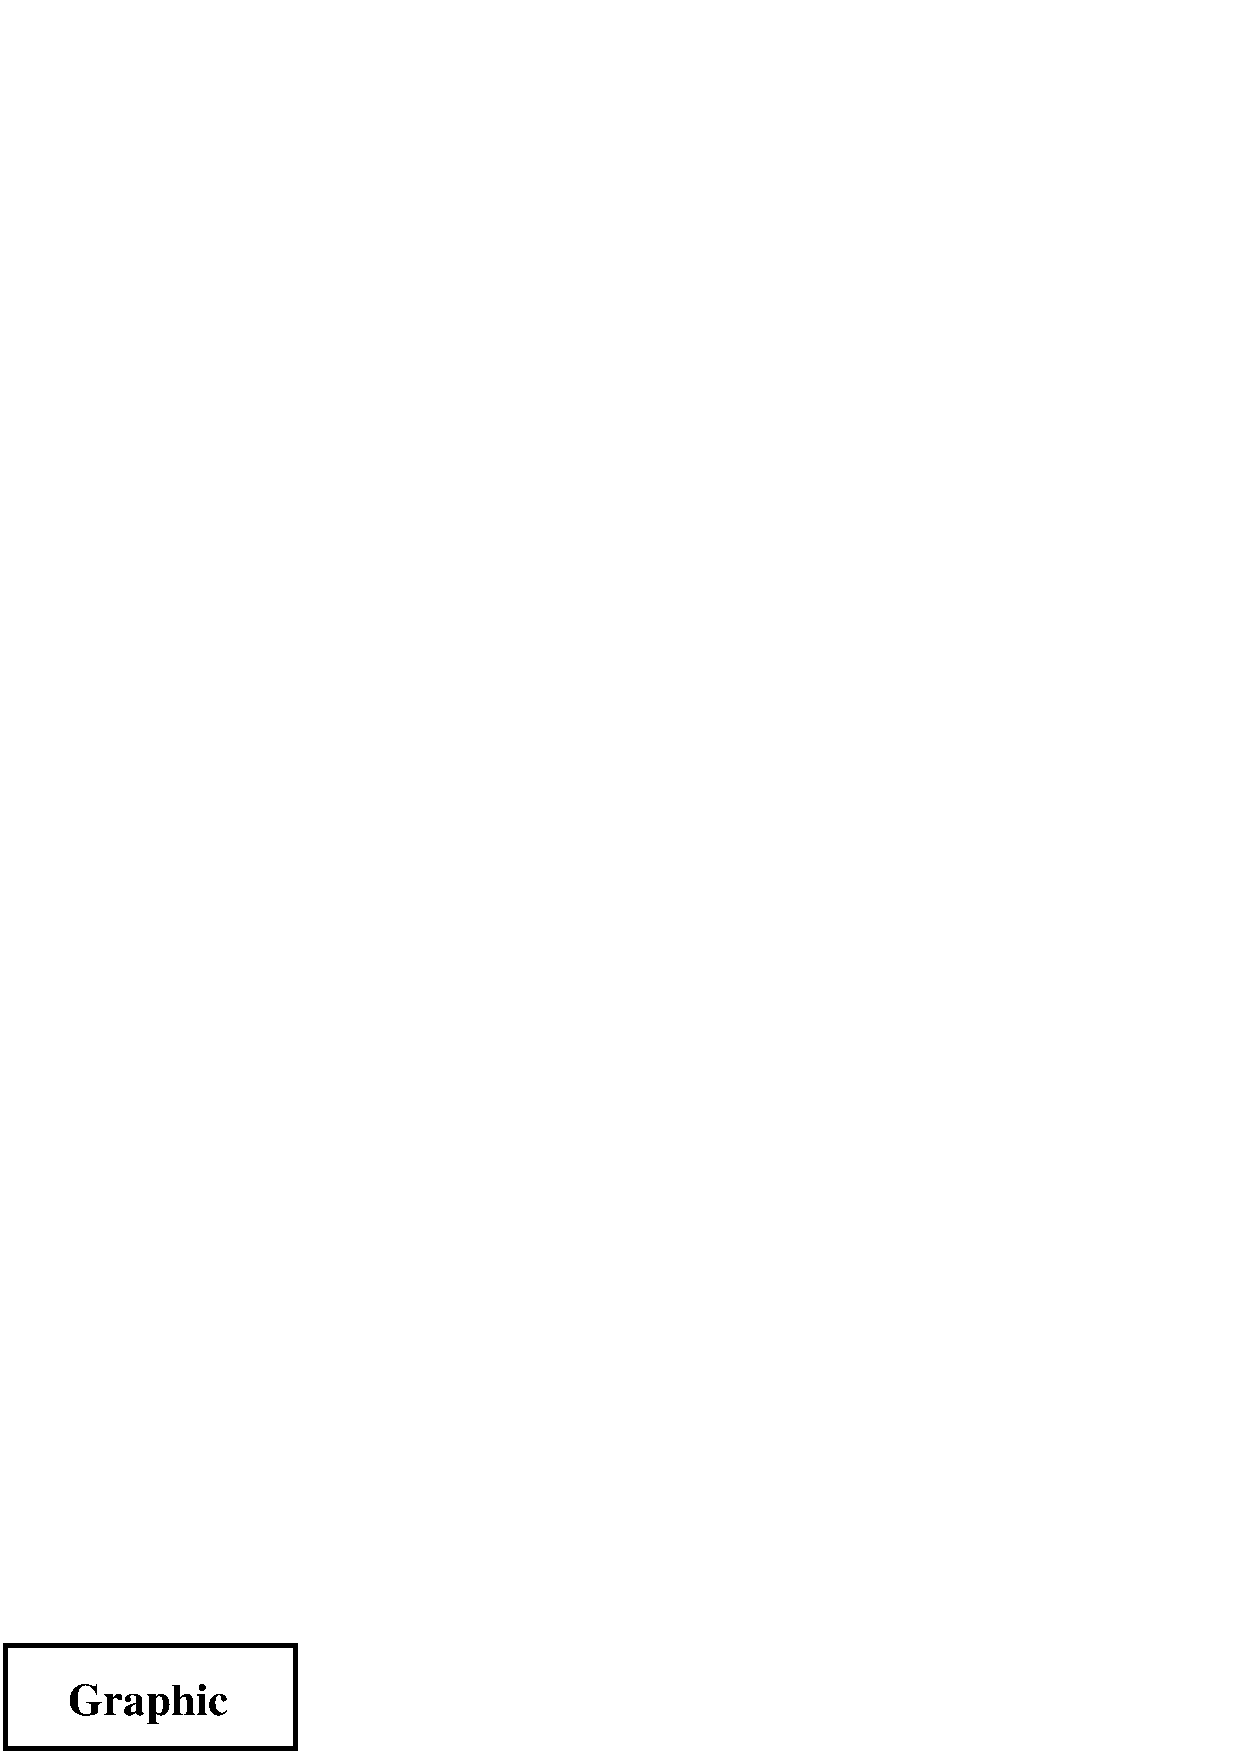
\includegraphics[width=1in,angle=-45]{graphic}
\end{minipage}
\end{center}
\end{lstlisting}
都得到图~\ref{fig:minipagesamp-1}~的结果。
在这两种情况下,小页的参考点都是图形的参考点(左下角)。
\begin{figure}
\begin{center}
	\begin{minipage}[t]{.25\linewidth}
		\centering
		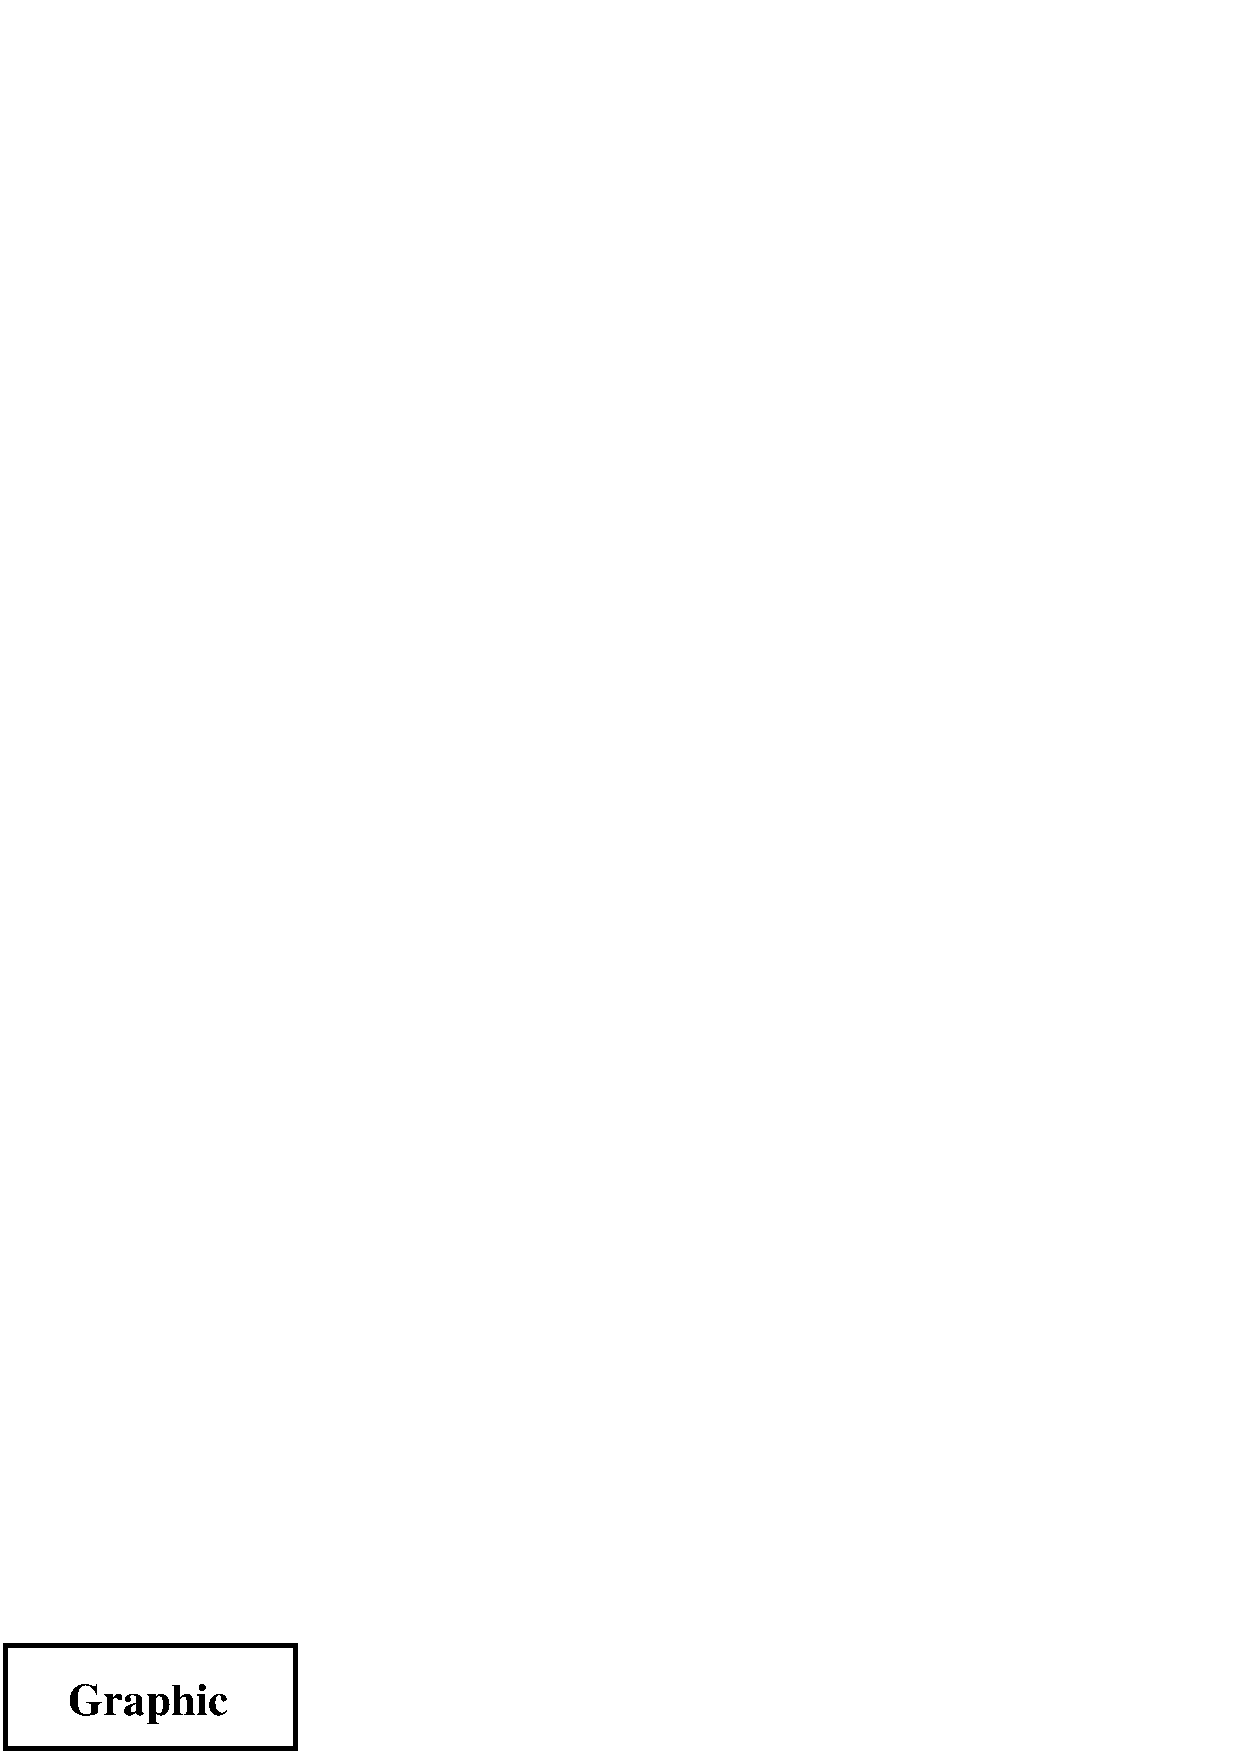
\includegraphics[width=1in]{graphic}
	\end{minipage}%
	\begin{minipage}[t]{.25\linewidth}
		\centering
		\includegraphics[width=1in,angle=-45]{graphic}
	\end{minipage}
\end{center}
\caption{带 minipage with \opt{[b]} or \opt{[t]} 选项的 \env{minipage} 环境}
\label{fig:minipagesamp-1}
\end{figure}

\subsubsection{小页的底部对齐}
让小页的底部对齐的一种方法是强制使小页的底部为其基线。
再次要注意的是,\env{minipage} 的 \opt{[b]} 选项效果是让小页最底行的基线作为小页的基线。

如果小页最底行正好是一条高和深都为零的线,
那么最后一行的参考点就是该行的底部,
这样 \opt{[b]} 选项就可使作为其基线。
类似地,如果在 \verb|\end{minipage}| 之前添加一条高度和深度为零的线,
那么 \opt{[b]} 选项就会使小页的底部作为小页的基线。
命令 \cmd{par}\cmdM{vspace}{0pt} 就可以产生这样高和深都为零的线段。
这时这条深度为零的线的基线就是小页的底部,
选项 \opt{[b]} 可以让小页的底部对齐了。例如:
\begin{lstlisting}
\begin{center}
\begin{minipage}[b]{.25\linewidth}
\centering
\includegraphics[width=1in]{graphic}
\par\vspace{0pt}
\end{minipage}%
\begin{minipage}[b]{.25\linewidth}
\centering
\includegraphics[width=1in,angle=-45]{graphic}
\par\vspace{0pt}
\end{minipage}
\end{center}
\end{lstlisting}
结果如图~\ref{fig:minipagesamp-2}。
\begin{figure}
\begin{center}
	\begin{minipage}[b]{.25\linewidth}
		\centering
		\includegraphics[width=1in]{graphic}
		\par\vspace{0pt}
	\end{minipage}%
	\begin{minipage}[b]{.25\linewidth}
		\centering
		\includegraphics[width=1in,angle=-45]{graphic}
		\par\vspace{0pt}
	\end{minipage}
\end{center}
\caption{底端对齐的小页环境}\label{fig:minipagesamp-2}
\end{figure}

\subsubsection{小页的顶部对齐}
当在小页的顶行加入一条高度和深度都为零的线段时,
使用 \opt{[t]} 选项使得小页的基线为它的顶部。
如果在并列的若干小页环境中都进行这样的操作,那么就可以使这些小页环境的顶端对齐。

命令 \cmdM{vspace}{0pt} 可以在小页的顶端插入一条高度和深度都为零的线段。
由于该条高度为零的线段的基线就位于小页的顶部,
现在使用 \opt{[t]} 选项就可以使得小页的顶部对齐了。例如:
\begin{lstlisting}
\begin{center}
\begin{minipage}[t]{.25\linewidth}
\vspace{0pt}
\centering
\includegraphics[width=1in]{graphic}
\end{minipage}%
\begin{minipage}[t]{.25\linewidth}
\vspace{0pt}
\centering
\includegraphics[width=1in,angle=-45]{graphic}
\end{minipage}
\end{center}
\end{lstlisting}
结果如图~\ref{fig:minipagesamp-3}~所示。
\begin{figure}
\begin{center}
	\begin{minipage}[t]{.25\linewidth}
		\vspace{0pt}
		\centering
		\includegraphics[width=1in]{graphic}
	\end{minipage}%
	\begin{minipage}[t]{.25\linewidth}
		\vspace{0pt}
		\centering
		\includegraphics[width=1in,angle=-45]{graphic}
	\end{minipage}
\end{center}
\caption{顶部对齐的小页环境}\label{fig:minipagesamp-3}
\end{figure}

这里小页的顶部是和当前基线对齐。
如果要求小页的顶部是和当前文本行的顶部对齐,
可用 \cmdM{vspace}{-\cmd{baselineskip}}。
  ~\verb+\vspace{-\baselineskip}+~来
相关专题参考~\cite[第~863--865~页]{Mittelbach2004}。


\section{两幅图像的堆叠}
本节描述如何堆叠两幅图像。
请注意这里没有检查确保顶层的图像是透明的。
如果顶层图像创建时使用非透明的背景,那么就会隐藏底层图像。

例如\footnote{
	尽管在这个例子中使用了两个 \file{eps} 图像,
	类似的代码也可以用于堆叠其它图像格式。
},
文件 \file{left.eps} 和 \file{right.eps} 包含的图像如图~\ref{fig:leftright} 所示。
使用如下命令
\begin{lstlisting}
\makebox[0pt][l]{\includegraphics{left.eps}}%
\includegraphics{right.eps}
\end{lstlisting}
就会堆叠两幅图像,如图~\ref{fig:leftrightoverlay} 所示。
堆叠两幅图像时,它们参考点(左下角)是重合的。
在这个例子中,两幅图像的自然大小是相同的,
所以不需要缩放就可以完全堆叠在一起。
其它的图像可能需要缩放
(使用 \cmd{includegraphics}、\cmd{scalebox} 或是 \cmd{resizebox} 等命令)
才能达到想要的堆叠效果。

如果没能理解 \cmd{makebox} 命令,这样的堆叠代码看起来就会显得有些不可思议。
实际上,\cmdOOM{makebox}{0pt}{l}{...} 命令会创建一个宽度为零的盒子。
当指定宽度时(这里是 \texttt{0 pt}),
那么排版算法就会分配这样宽度的水平空间,而不管其中内容的实际宽度是怎样。
这样,对于一个内容居左的宽度为零的盒子,
之后的\LaTeX{} 对象的排版效果就是覆盖在该盒子之上。

\begin{figure}
	\centering
	\includegraphics{left.eps}
	\caption{两幅图像的内容}\label{fig:leftright}
\end{figure}
\begin{figure}
	\centering
	\makebox[0pt][l]{\includegraphics{left.eps}}%
	\includegraphics{right.eps}
	\caption{两幅堆叠的图像}\label{fig:leftrightoverlay}
\end{figure}

\subsection{Overpic 宏包}
另一种堆叠图像的方法是使用 \pkgi{overpic} 宏包。
该宏包定义了一个图形环境,使得大小就是插图的尺寸大小。
相关细节参考 \pkg{overpic} 宏包文档~\cite{overpic-doc}。


\section{使用子目录}\label{sec:subdir}

当需要大量的图形文件时,你可能希望将它们存放到一个子目录下。
例如,假设子目录的名字叫 \file{sub},这时你试图用如下的命令来插入图形 \file{file.eps}。
\begin{lstlisting}
\includegraphics{sub/file.eps}
\end{lstlisting}

尽管这种用法在大多数 Unix 和 DOS 下的 \TeX{} 发行版里工作正常,它却有以下的问题:
\begin{description}
	\item [效率不高]
	
	每当 \TeX{} 打开一个文件,该文件名就被存入 TeX{} 的内存中。
	当打开大量的文件时,内存空间减少会导致内存池大小的错误(见第~\ref{ssec:poolspace}~节)。
	显式地给出子目录名增加了文件名的长度,进而加重这种池空间问题。
	
	\item [通用性差]
	
	\LaTeX{} 的一大优势就是它的文件能在任何操作系统平台上使用。
	然而,在文件名中包括子目录名会使文件依赖于操作系统。
	如果不作明显的改变,上面的例子就无法在 VMS 或 Macintosh 上使用。
\end{description}
实际上除了直接在文件名中使用子目录外,还有两种选择。
\begin{enumerate}
	\item 最好的方法是将子目录加到 \TeX{} 搜索路径中(见第 \ref{ssec:texpath} 节)。
	\item 另外一种办法是用 \cmdi{graphicspath} 命令来指明所用的子目录
	(见第~\ref{ssec:graphpath}~节)。不过,这比前一种方法的效率要低不少。
\end{enumerate}

上述两种方法都将使 \cmd{includegraphics} 自动搜索图形子目录,
故可在使用
\begin{lstlisting}
\includegraphics{file.eps}
\end{lstlisting}
来替代
\begin{lstlisting}
\includegraphics{sub/file.eps}
\end{lstlisting}

\subsection{\TeX{}~搜索路径}\label{ssec:texpath}

因为不同的\TeX{} 发行版设置搜索路径的方法不完全一样,
所以很难提供一个普遍适用的范例。
本节所用的例子基于 Unix 下的 web2c/te\TeX{}。
尽管稍有不同,但其它的 \TeX{} 发行版也大致采用相似的策略。

对 Unix 下的 web2c/te\TeX{} 而言,
改变 \TeX{} 的搜索路径可通过设置环境变量 \file{TEXINPUTS} 来实现。
如使用 \prgname{csh},命令
\begin{lstlisting}[language=csh]
setenv TEXINPUTS /dir1:/dir2:
\end{lstlisting}
会使 \TeX{} 在搜索缺省的目录前先搜索 \file{/dir1} 和 \file{/dir2}。
如果省掉最后的冒号 \texttt{:},
那么在搜索完 \file{/dir1} 和 \file{/dir2} 后 \TeX{} 将不再搜索缺省的目录。
如设
\begin{lstlisting}[language=csh]
setenv TEXINPUTS :/dir1:/dir2
\end{lstlisting}
则使 \TeX{} 在搜索缺省的目录后再搜索 \file{/dir1} 和 \file{/dir2}。
而
\begin{lstlisting}[language=csh]
setenv TEXINPUTS /dir1::/dir2
\end{lstlisting}
则使 \TeX{} 在搜索 \file{/dir1} 后接下来搜索缺省的目录,
最后再搜索\file{/dir2}。

在一个目录后面加上 \file{//} 使得此目录下的所有子目录都将被搜索。
例如:
\begin{lstlisting}[language=csh]
setenv TEXINPUTS /dir1//:/dir2:
\end{lstlisting}
会使 \TeX{} 搜索 \file{/dir1} 的所有子目录(以及子目录的子目录,等等)。
使用 \file{//} 要小心,如果一目录下的文件和子目录特别多的话,
它会使 \TeX{} 的搜索速度变得很慢。

若使用 \prgname{sh},可用命令
\begin{lstlisting}[language=sh]
TEXINPUTS="/dir1:/dir2:"; export TEXINPUTS
\end{lstlisting}
来设置环境变量 \file{TEXINPUTS}。

当 \LaTeX{} 在 \TeX{} 搜索路径中寻找文件时,不会将目录名也写到 \file{dvi} 文件中。
对于旧版本的 \prgname{dvips} 和 \prgname{xdvi} 而言,
由于没有搜索\TeX{}~的搜索路径的功能,
因此,可能会找不到该文件(见第~\ref{ssec:dvips}~节)。









\subsection{临时改变 \TeX{} 的搜索路径}\label{ssec:temptexpath}

本节讲述如何使用 Unix shell 临时修改 \TeX{} 搜索路径,
以便寻找特定项目的图像文件。
用户可以为每一个 \LaTeX{} 项目创建各自不同的 shell 脚本,
每一个脚本指定的路径对于该项目来说是唯一的。

例如,假设用户正在写一篇期刊文章,
想要创建一个 shell 脚本 \verb|latex_paper| 来代替 \prgname{latex} 命令。
在 Unix 搜索路径上创建一个文件 \verb|latex_paper|,其中包含如下内容
\begin{lstlisting}[language=sh]
#!/bin/sh
TEXINPUTS= ~/PAPER/SUB1/:~/PAPER/SUB2/:$TEXINPUTS latex $@
\end{lstlisting}
使用如下命令将该文件转成可执行文件
\begin{lstlisting}[language=sh]
chmod u+x latex_paper
\end{lstlisting}

设置好之后,输入
\begin{lstlisting}[language=sh]
latex_paper file.tex
\end{lstlisting}
就会在 \file{TEXINPUTS} 的开头添加 \file{~/PAPER/SUB1/:~/PAPER/SUB2/},
之后用 \prgname{latex} 运行 \file{file.tex},
就可以搜索 \file{~/PAPER/SUB1/} 和 \file{~/PAPER/SUB2/} 子目录下的任何图像文件。

类似地,还需要写一个 \verb|dvips_paper| 脚本,
以便让 \prgname{dvips} 在 \file{dvi} 转 \file{ps} 过程中可以搜索到图像文件。

\subsection{图形文件搜索路径}\label{ssec:graphpath}
缺省地, \LaTeX{} 在 \TeX{} 搜索路径中寻找图形文件。
除此之外, \LaTeX{} 还会搜索由 \cmdi{graphicspath} 给出的目录。
例如:
\begin{lstlisting}
\graphicspath{{dir1/}{dir2/}}
\end{lstlisting}
告诉 \LaTeX{} 也从目录 \file{dir1/} 和 \file{dir2/} 下寻找图形文件。
对 Macintosh 系统来说,上面的命令改为:
\begin{lstlisting}
\graphicspath{{dir1:}{dir2:}}
\end{lstlisting}

很重要的一点是,搜索由 \cmd{graphicspath} 给出的目录要比由 \file{TEXINPUTS} 给出的目录慢的多。
更进一步说,搜索由 \cmd{graphicspath} 给出的目录要占用一定的池空间
(见第~\ref{ssec:poolspace}节)。
鉴于 \cmd{graphicspath} 效率不高,所以一般不推荐使用这一命令,
最好的办法就是将要使用的目录加到 \TeX{} 搜索路径中去(见第~\ref{ssec:texpath}~节)。


\subsection{节约池空间}\label{ssec:poolspace}

\TeX{} 为其内部的字符串传递保留了一部分内存空间,称为\emph{池空间}(\emphi{pool space})。
每当 \TeX{} (试图)打开打开一文件,就会有一部分池空间按被永久性分配。
当打开很多文件时,这种内存的占用会导致 \TeX{} 耗光它的池空间,产生如下的错误讯息:
\begin{Verbatim}[xleftmargin=1cm]
! TeX capacity exceeded, sorry [poolsize=72288]
\end{Verbatim}

由于占用的池空间与文件名的长度有关,
所以其中带有子目录的文件名会加重该问题。

除了最新版的基于 web2c 的 \TeX{} 软件和一些商业软件外,
增加池空间的唯一办法就是重新编译 \TeX{}。
所幸的是,通常用下面这些节约池空间的办法就可以解决问题。

\begin{itemize}
\item 避免用过长的文件名。

\item 不要把子目录名包括进来
	\begin{lstlisting}
	\includegraphics{images/file.eps}
	\end{lstlisting}
	取而代之的是将子目录加到 \TeX{} 搜索路径中或不要把图形文件放在子目录下。
	
\item 不要使用 \cmd{graphicspath} 命令。如下代码
	\begin{lstlisting}
	\graphicspath{{dir1/}{dir2/}}
	...
	\includegraphics{file.eps}
	\end{lstlisting}
	将使 \cmd{includegraphics} 命令试图打开下列文件:
	\begin{Verbatim}[xleftmargin=1.5cm]
	file.eps
	dir1/file.eps
	dir2/file.eps
	\end{Verbatim}
	每一次打开文件的尝试都会消耗池空间。
	应该用更改 \TeX{} 搜索路径的办法来替代使用命令 \cmd{graphicspath}。
	
\item 给出全部的文件名,不要省略文件的扩展名(例如 \file{.eps})。
	在缺省的 \cmd{DeclareGraphicsExtensions} (第~\ref{ssec:deextension} 节)定义下,命令
	\begin{lstlisting}
	\includegraphics{file}
	\end{lstlisting}
	将使 \cmd{includegraphics} 命令试图打开下列文件:
	\begin{Verbatim}[xleftmargin=1.5cm]
	file.eps
	file.ps
	file.eps.gz
	file.ps.gz
	file.eps.Z
	\end{Verbatim}
	若是再加上使用~\cmd{graphicspath},会导致效率特别低。
	
	最好将 \cmd{DeclareGraphicsExtensions} 中定义的扩展名列表减到最小,
	这样在使用省略扩展名的文件时会好些。
\end{itemize}

请注意,\cmd{includegraphics} 命令只会在打开或试图打开文件时消耗池空间。
由于 \cmd{includegraphics} 命令打开文件的目的只是为了确定图像的 BoundingBox,
因此,为了阻止池空间消耗,一种有效但却不那么方便的的方法就是,
使用 \cmd{includegraphics} 命令的 \opt{bb} 选项指定 BoundingBox 参数值(见表~\ref{tab:opt})。


\section{在 DVIPS 中使用压缩EPS文件和非 EPS 文件}\label{sec:dvips-noneps}

正如第~\ref{sec:intro} 节所述,在 \prgname{dvips} 模式下,
\LaTeX{} 图像插入的任务是由 \file{dvi} 程序负责。
这就意味着,\LaTeX{} 文档可以使用任何 \file{dvi} 程序支持的图像格式。
尽管事实上所有的 \file{dvi}-\file{ps} 转换程序都支持 \file{eps} 图像,
但几乎没有转换程序支持非 \file{eps} 图像。
所以,在 \prgname{dvips} 模式下,
要使用非 \file{eps} 图像需要将其转成 \file{eps} 格式。
而这可以有两种办法。
\begin{description}
	\item[提前转换] 在 \file{dvi}-\file{ps} 转换之前,
	使用图像转换程序将非\file{eps} 图像转成\file{eps} 格式。
	保存的 \file{eps} 格式可以用于接下来的 \file{dvi}-\file{ps} 过程。
	
	\item[实时转换] 在 \file{dvi}-\file{ps} 过程中,
	\file{dvi}-\file{ps} 转换程序调用一个图像转换程序,
	使得图像转换的结果通过管道传回 \file{dvi}-\file{ps} 程序,最后插入到 \file{ps} 文件中。
\end{description}
提前转换的缺点是需要存储图像文件的 \file{eps} 版本。
尽管“实时转换”方法不需要额外存储,
但需要在每一次执行 \file{dvi}-\file{ps} 程序时都进行重复的图像转换计算。
所以这里需要在速度和存储之间进行权衡。
不过大部分用户偏向“提前转换”带来的速度优势。

与直接整合图像转换指令不同,\prgname{dvips} 提供了一种调用外部转换程序的机制
\footnote{
	这种机制需要操作系统支持管道功能。}。
这可以通过在 \LaTeX{} 中使用 \cmd{DeclareGraphicsRule} 的命令选项来完成。
这种方法比直接的图像转换支持更方便灵活,因为图像转换和 \file{dvi}-\file{ps} 过程是分开的,
因此,用户可以选择自己想用的图像转换程序。

当在支持管道的操作系统中使用 \prgname{dvips} 时\footnote{
	例如,Unix 支持管道而 DOS 则不支持},
可以使用 \cmd{DeclareGraphicsRule} (见第~\ref{ssec:derule} 节)指定在文件上执行的操作。
若为解压缩命令,则可允许使用压缩的图形文件。
若为图形格式转换命令,则可允许使用非 \file{eps} 图形文件。
当使用不支持管道的操作系统时,这种即时转换的命令是不允许的,
这时只好将所有的图形文件都存为非压缩的 \file{eps} 格式。

考虑到目前为止 \file{dvi}-\file{ps} 转换程序中只有 \prgname{dvips} 具有这种功能,
本节所介绍的内容都需要 \prgname{dvips} 的支持。
使用者需要在使用 \pkg{graphicx} 宏包时设定使用 \opt{dvips} 选项。
这可以通过在 \cmd{documentclass} 中指定 \opt{dvips} 全局选项进行全局设定:
\begin{lstlisting}
\documentclass[dvips,11pt]{article}
\end{lstlisting}
或者在 \cmd{usepackage} 中设定 \pkg{graphicx} 的使用 \opt{dvips} 选项为:
\begin{lstlisting}
\usepackage[dvips]{graphicx}
\end{lstlisting}
推荐使用第一种方法,因为它将 \opt{dvips} 这一选项传递给所有的宏包。


\subsection{压缩 EPS 文件的例子}\label{ssec:compresseps}
使用压缩 \file{eps} 文件的步骤是:
\begin{enumerate}
	\item 创建一个 \file{eps} 文件(比如说 \file{file1.eps})。
	\item 将它的 BoundingBox 存放到另外一文件中(~\file{file1.eps.bb})。
	\item 压缩  \file{eps}  文件,比如在很多平台上用命令:
	\begin{lstlisting}[language=bash]
	gzip -9 file1.eps
	\end{lstlisting}
	得到压缩文件 \file{file1.eps.gz}。这里 \opt{-9}(或者 \opt{-best}) 选项表示最佳压缩。
	\item 在 \cmd{includegraphics}前声明适当的 \cmd{DeclareGraphicsRule} 命令。
	使得 \LaTeX{} 知道如何处理特殊后缀的文件(见第~\ref{ssec:derule}~节)。例如:
\begin{lstlisting}
\documentclass[dvips]{article}
\usepackage{graphicx}
\begin{document}
\DeclareGraphicsRule{.eps.gz}{eps}{.eps.bb}{`gunzip -c #1}
\begin{figure}
\centering
\includegraphics[width=3in]{file1.eps.gz}
\caption{压缩的 EPS 图像}
\label{fig:compressed:eps}
\end{figure}
\end{document}
\end{lstlisting}
	在这个特殊的例子里,\cmd{DeclareGraphicsRule} 实际上是可以省略的,
	因为在 \file{dvips.def} 已经预定义过了。
	如果使用另外一个解压缩程序或文件名后缀,那么 \cmd{DeclareGraphicsRule} 是不能少的。
	例如 BoundingBox~存放到文件 \texttt{file.bb} 中,
	则相应的 \cmd{DeclareGraphicsRule} 应为:
\begin{lstlisting}
\DeclareGraphicsRule{.eps.gz}{eps}{.bb}{`gunzip -c #1}
\end{lstlisting}
\end{enumerate}


\subsection{非 EPS 图形文件}\label{ssec:noneps}

EPS~格式的图形文件可以很容易的插入到~\LaTeX{}~文件中,
而非~EPS~格式的图形文件(\file{gif}、\file{tiff}、\file{jpeg}、\file{pict} 等)则不是将插图命令中的文件名替换一下就可以的。
一个简单的解决方法是检查一下生成该图像的应用程序是否也可以输出 \file{eps}。
如果不是的话,就必须用图像转换程序(见第~\ref{ssec:convertor} 节)将其转成 PostScript。
尽管使用非 \file{eps} 格式的图形文件不如 \file{eps} 图形文件简单方便,
但由于它们可能比 \file{eps} 文件要小,而一些绘图软件也不能生成~EPS~文件,
所以有时还是希望在 \file{dvi} 文件转换为 \file{ps} 文件时再对其进行图像格式转换。
如果使用 \prgname{dvips},这种即时转换的命令可用 \cmd{DeclareGraphicsRule}来给出。
例如用这种方法将 \file{file2.gif} 插入到 \LaTeX{} 文档中需要以下几步:
\begin{enumerate}
	\item 找到一个支持命令行方式的 \file{gif} 到 \file{eps} 的转换工具
	(假设为 \prgname{gif2eps})。
	\item 创建一个指定 \file{file2.gif} 自然大小的 BoundingBox 文件。
	为此,
	\begin{enumerate}
		\item 如果 PostScript 文件包含 BoundingBox 行,
		将此行保存到文件 \file{file2.gif.bb}
		\item 如果 PostScript 文件不包含 BoundingBox 行,
		用 \verb|ebb file2.gif| 直接得到 BoundingBox 文件\footnote{
			\prgname{ebb} 是 \prgname{dvipdfm} 中的一个应用程序,
			用来计算非\file{eps} 图形文件的 BoundingBox。——旧译本}。
		\item 将 \file{file2.gif} 转成PostScript。
		如果 PostScript 文件包含 BoundingBox 行,则将此行保存到文件 \file{file2.gif.bb};
		否则,可按照第~\ref{ssec:pstoeps}~节的方法来计算 BoundingBox,
		并将所得到的结果放在 \file{file2.gif.bb} 中的 \verb|%%BoundingBox|后。
		然后将 PostScript 文件删除。
	\end{enumerate}
	\item \LaTeX{} 文件中,在 \cmd{includegraphics} 命令前,加入图形规则:
	\begin{lstlisting}
	\DeclareGraphicsRule{.gif}{eps}{.gif.bb}{`gif2eps #1}
	\end{lstlisting}
\end{enumerate}
当遇到 \cmdM{includegraphics}{file.gif} 时,
\LaTeX{} 会从 \file{file.gif.bb} 中读取 BoundingBox,
并告诉 \prgname{dvips} 使用 \prgname{gif2eps} 来将 \file{file.gif} 转为 \file{eps} 文件。


\subsection{GIF 的例子}\label{ssec:gifexample}
由于插入非 \file{eps} 格式的图形所需的命令依赖于操作系统和图形格式转换程序,
在此提供两个 Unix 系统下常用的转换程序的例子。

\begin{lstlisting}
\DeclareGraphicsRule{.gif}{eps}{.gif.bb}{`convert #1 'eps:-' }
\begin{figure}
\centering
\includegraphics[width=3in]{file2.gif}
\caption{GIF Graphic}
\end{figure}
\end{lstlisting}
这里使用 \prgname{convert}命令(包含在 ImageMagick 中)将\file{gif} 转为 \file{eps}。
而命令:
\begin{lstlisting}[language=bash]
convert file2.gif 'eps:-'
\end{lstlisting}
将 \file{file2.gif} 转为\file{eps}格式(“\opt{eps:}”选项)并输出到标准输出(“\opt{-}”指示符)。

另一方法是使用 \prgname{ppm} 组件的 \prgname{giftoppm}、\prgname{ppmtopgm} 和 \prgname{pgmtops} 程序
将 \file{gif} 通过 \file{ppm} 和灰度 \file{pgm} 格式最终转为\file{eps}。
在Unix中,使用如下 \cmd{DeclareGraphicsRule} 命令可以将这些程序用管道连接起来:
\begin{lstlisting}
\DeclareGraphicsRule{.gif}{eps}{.gif.bb}{`giftoppm #1 | ppmtopgm | pgmtops}
\end{lstlisting}


\subsection{\TeX{} 搜索路径和 dvips}\label{ssec:path-dvips}

当 \LaTeX{} 遇到\cmd{includegraphics} 命令时,
会首先在当前目录下搜寻图形文件。
如果找不到所需的文件,\LaTeX{} 将按照 \TeX{} 搜索路径来寻找。
当 \file{dvi} 文件转为PostScript文件时,\prgname{dvips} 也是同样地顺序来搜寻图形文件。
这不会有什么问题。
然而,如果用 \cmd{DeclareGraphicsRule} 定义了一个实时转换的命令,
那么此命令将会阻止 \prgname{dvips} 在 \TeX{} 搜索路径中寻找图形文件。

例如:
\begin{lstlisting}
\DeclareGraphicsRule{.eps.gz}{eps}{.eps.bb}{`gunzip -c #1}
\end{lstlisting}
指定对后缀为 \texttt{.eps.gz} 的文件使用命令 \texttt{gunzip -c}。
假设用下面的命令来插入图形文件,
\begin{lstlisting}
\includegraphics{file.eps.gz}
\end{lstlisting}
如果 \file{file.eps.gz} 和 \file{file.eps.bb} 在当前目录下的话,
那么不需要路径搜索,一切没有问题。
\LaTeX{} 会使用 \file{file.eps.bb} 而 \prgname{dvips} 则执行 
\verb|gunzip -c file.eps.gz| 来解压缩文件。

但是,如果 \file{file.eps.gz} 和 \file{file.eps.bb} 不在当前目录就会有问题。
假设在目录 \file{/a/b/c/} 下(并且该目录已加到 \TeX{} 搜索路径中)。
\LaTeX{} 通过搜索路径仍然能够找到 \file{/a/b/c/file.eps.bb},
但 \prgname{dvips} 在执行\verb|gunzip -c file.eps.gz| 就会出问题。
因为 \prgname{gunzip} 找不到文件 \file{file.eps.gz}。

如果 \TeX{} 发行版使用了 \prgname{kpathsea} 库(比如 te\TeX{} 发行版),
这个问题可用定义下面的图形规则来解决。
\begin{lstlisting}
\DeclareGraphicsRule{.eps.gz}{eps}{.eps.bb}%
{`gunzip -c `kpsewhich -n latex tex #1`}
\end{lstlisting}
这里使用 \prgname{kpsewhich}\index{kpsewhich@\textsf} 为 \prgname{gunzip} 寻找文件。
\begin{lstlisting}[language=bash]
`kpsewhich -n latex tex #1
\end{lstlisting}
会使得 \prgname{dvips} 在 \TeX{} 搜索路径中寻找压缩图形文件,
然后把文件的全名(包括目录名)附加到 \texttt{gunzip -c} 命令后,
这样即使压缩图形文件不在当前目录下,\prgname{gunzip} 也可对其进行操作。

虽然上面给出的新的图形规则可以放在每个 \LaTeX{} 文件的开头,
但是更方便的用法是把如下代码放到 \file{graphics.cfg} 文件中:
\begin{lstlisting}
\AtEndOfPackage{%
\DeclareGraphicsRule{.eps.gz}{eps}{.eps.bb}%
{`gunzip -c `kpsewhich -n latex tex #1`}}
\end{lstlisting}
并且保留 \cmdM{ExecuteOptions}{dvips} 这一行。


\section{在图像上添加\LaTeX{}标记}\label{sec:graphics-text}

\subsection{PSgrag 宏包}\label{ssec:psfrag}

目前很多绘图和分析软件都可以输出\file{eps}格式的图形,
但是它们大都不能像 \LaTeX{} 一样支持符号和公式。
\pkgi{PSfrag} 宏包允许用 \LaTeX{} 的文本和公式来替代 \file{eps} 图形文件中的字符。

\pkg{PSfrag} 3.0 是1996年发布的完全重写版本。
以前的版本则需要借助预处理程序(\prgname{ps2frag} 或 \prgname{ps2psfrag})
来识别和标记 \file{eps} 图形文件中的文本。
而\pkg{PSfrag} 3.0 不需要借助预处理程序,
也不需要像 \prgname{perl} 或 \prgname{ghostscript} 等外部程序。
\pkg{PSfrag} 3.0 只需要较近版本的 \LaTeX{} 和图形宏包套件。
参考文献 \cite{psfrag-doc} 给出了\pkg{PSfrag} 3.0 的详细说明。

\pkg{PSfrag} 的另一优势是支持压缩的 \file{eps} 图形。
不过,\cmd{tex} 命令(见第~\ref{sssec:latextext}~节)
不能用于在压缩的 \file{eps} 图形中嵌入 \LaTeX{} 文本。

使用\pkg{PSfrag} 的步骤是:
\begin{enumerate}
	\item 在 \LaTeX{} 文档的导言区中加入:\cmdM{usepackage}{psfrag}。
	\item 在文档中使用 \cmd{psfrag} 命令来指明要替换的 \file{eps} 文本以及取而代之的 \LaTeX{} 字符串。
	同一环境下之后的任何 \cmd{includegraphics} 命令中会执行这些替换。
	\item 像通常一样使用 \cmd{includegraphics} 即可。
\end{enumerate}

\cmdi{psfrag} 命令的用法如下:
\begin{lstlisting}
\psfrag{PStext}[posn][PSposn][scale][rot]{text}
\end{lstlisting}
其中选项说明见表~\ref{tab:psfrag}。

选项 \opt{posn} 和 \opt{PSposn} 可以是第~\pageref{fig:rotatepoint}~页图~\ref{fig:rotatepoint}~所示的~12~个点中的一个(例如 \opt{[tl]}、\opt{[br]}、\opt{[cc]})。
如果没有给出,默认点是 \opt{[Bl]}。
缺失字母默认为 \opt{c},例如 \opt{[]} 和 \opt{[c]} 都等价于 \opt{[cc]},
\opt{[l]} 等价于 \opt{[lc]}。
可参考 \cite{psfrag-doc} 中各种位置组合的例子。

\begin{table}
\centering
\caption{\pkg{PSfrag} 选项}\label{tab:psfrag}
\begin{tabular}{>{\ttfamily}lp{0.7\textwidth}}
\toprule
{PStext} & \file{eps} 图形中被替换的文本。\\
\midrule
{posn}  & (可选项,缺省为~\opt{[Bl]})放置点相对于 \LaTeX{} 文本的参考位置。 \\
\midrule
{PSposn} & (可选项,缺省为~\opt{[Bl]})放置点相对于现有 \file{eps} 文本的参考位置。 \\
\midrule
{scale} & (可选项,缺省为1) \LaTeX{} 文本的缩放因子。
	为得到最好的效果,建议不使用这一选项,
	而使用 \cmd{small} 和 \cmd{large} 等 \LaTeX{} 字体命令。\\
\midrule
{rot}  & (可选项,缺省为零)当给出一个角度时,
	此角度即为新的 \LaTeX{} 文本相对于旧的 \file{eps} 图形中文本的角度。
	它以度为单位并且逆时针方向为正。
	此选项特别适用于应用软件只能生成包含水平方向文本的 \file{eps} 图像的情形。\\
\midrule
{text} &  用来插入 \file{eps} 图像的 \LaTeX{} 文本。
	如同通常的~\LaTeX{}~文本,数学公式必须放在美元符号对
	中。如 \verb+$\frac{1}{2}$+ 或 \verb+$x^2$+。\\
\bottomrule
\end{tabular}
\end{table}

需要注意的是 \cmd{psfrag} 只匹配整个字符串,例如下面的命令
\begin{lstlisting}
\psfrag{pi}{$\pi$}
\end{lstlisting}
用 $\pi$ 替换 \opt{pi},但不会影响其它像 \texttt{pi/2} 或 \texttt{2pi} 这样的 \file{eps} 字符串。对于必须各自使用 \cmd{psfrag} 命令。

如果所替换的 \file{eps} 字符串不是完整的置于一个 PostScript命令中,
\marginpar{间距问题}
那么 \cmd{PSfrag} 将不起作用。
在一些应用软件生成的 \file{eps} 图形中,为达到特殊的字符间距,
将一字符串分隔为几个子串或单个的字符。
例如,Corel Draw 可以用如下的 \file{eps} 代码来放置字符串“Hello World”:
\begin{Verbatim}[xleftmargin=1cm]
0 0 (Hello W) @t
1080 0 (orld) @t
\end{Verbatim}
由于 \pkg{PSfrag} 将其视为是两个不相干的字符串“Hello W”和“orld”,
所以任何对“Hello World”的替换都不起作用。
如果不能在应用软件中手动取消这种对字符间距的处理,
一般可以使用 Courier 或其它等宽字体来阻止这种情况\footnote{%
	为了避免字符间距,可能需要在创建文本之前设置Courier字体。
	先穿件文本在将其转成Courier字体可能仍然会有字符间距。}。
如果确实无法避免这种情况,那么只能对单个字符进行替换。

\subsubsection{PSfrag 使用例\#1}\label{sssec:psfragex1}

命令
\begin{lstlisting}
\includegraphics{pend.eps}
\end{lstlisting}
只是插入 \file{eps} 图形而没有任何 \pkg{psfrag} 替换,见图~\ref{fig:nopsfrag}。
而下面的命令
\begin{lstlisting}
\psfrag{q1}{$\theta_1$}
\psfrag{q2}{$\theta_2$}
\psfrag{L1}{$L_1$}
\psfrag{L2}{$L_2$}
\psfrag{P1}[][]{$P_1$}
\psfrag{P2}[][]{\large $P_2$}
\includegraphics{pend.eps}
\end{lstlisting}
在插入 \file{eps} 图形的同时使用 \pkg{psfrag} 对 \file{eps} 图形中的字符串进行替换,
见图~\ref{fig:psfragex1}。
前四个 \cmd{psfrag} 命令中,新的 \LaTeX{} 字符串的左基线点对应于旧的 \file{eps} 字符串的左基线点,
后面两个 \cmd{psfrag} 命令中使用 \opt{[][]} 选项使得新的 \LaTeX{} 字符串的中心对应于旧的 \file{eps} 字符串的中心。
注意并不是所有的 \file{eps} 字符串都被替换,
如在图~\ref{fig:psfragex1}~中 \texttt{N} 就没有被替换。

\begin{figure}
\begin{minipage}[t]{.5\textwidth}
\vspace{0pt}
\centering
\includegraphics[width=.9\textwidth]{pend}
\caption{Without PSfrag Replacement}\label{fig:nopsfrag}
\end{minipage}%
\begin{minipage}[t]{.5\textwidth}
\vspace{0pt}
\centering
\ifxetex
\includegraphics[width=.9\textwidth]{psfrag-ex1}
\ifpdf
\includegraphics[width=.9\textwidth]{psfrag-ex1}
\else
\ifdvipdfm
\includegraphics[width=.9\textwidth]{psfrag-ex1}
\else
\psfrag{q1}{$\theta_1$}
\psfrag{q2}{$\theta_2$}
\psfrag{L1}{$L_1$}
\psfrag{L2}{$L_2$}
\psfrag{P1}[][]{$P_1$}
\psfrag{P2}[][]{\large $P_2$}
\includegraphics[width=.6\textwidth]{pend.eps}
\fi
\fi
\fi
\caption{With PSfrag Replacement}\label{fig:psfragex1}
\end{minipage}
\end{figure}
===============================================================
\subsubsection{Psfrag~~使用例二}\label{sssec:psfragex2}

这个例子演示了~\ci{shortstack}, \ci{colorbox}~和~\ci{fcolorbox}~等命令如
何与~\cmd{psfrag}~一起使用。

\begin{description}
\item[\cmd{shortstack}] 这一命令允许将文本竖直放置,每行用~\verb+\\+~
     分开。可用来使用多行文本替换~EPS~图中的一行文本。
\item[\cmd{colorbox}] \pai{color}~宏包所提供的一个命令,它在所作用的
     对象背后放置一长方形的彩色区域作为背景。此背景超出对象的部分的大小
     由长度~\ci{fboxsep}~控制。例如:
     \begin{Verbatim}[formatcom=\color{VerbatimColor}\CJKfamily{kai}]
         \colorbox{yellow}{文本}
     \end{Verbatim}
     在{\colorbox{yellow}{\CJKfamily{kai}文本}}后放置了一长方形的黄色背景。
     有关~\cmd{colorbox}~的详细说明可参考文献~\cite{grfguide}。

     在使用~\textsf{PSfrag}~时,~\cmd{colorbox}~常常用来放置那些由于
     线条或阴影而被遮挡的文本。通过将这些文本的背景色设为白色,防止
     它们被图形所遮挡。
\item[\cmd{fcolorbox}] 这一命令(也由~\textsf{color}~宏包所提供)与
     ~\cmd{colorbox}~类似,只是为背景加上了一个边框。如命令
     \begin{Verbatim}[formatcom=\color{VerbatimColor}\CJKfamily{kai}]
         \fcolorbox{black}{yellow}{文本}
     \end{Verbatim}
     在{\fcolorbox{black}{yellow}{\CJKfamily{kai}文本}}后放置了一长方形的
    带有黑色边框的黄色背景。

     这里边框的宽度由~\ci{fboxrule}~控制,边框和对象之间的间隔大小
     则由~\cmd{fboxsep}~控制。
\end{description}

\begin{figure}
\hspace{-1.5cm}
\begin{minipage}[b]{.7\textwidth}
\centering
\includegraphics[width=.6\textwidth]{mass}
\caption{Without PSfrag Replacement}\label{fig:nopsfragex1}
\par\vspace{0pt}
\end{minipage}%
\hspace{-3cm}
\begin{minipage}[b]{.7\textwidth}
\ifpdf
\centering
\includegraphics[width=.6\textwidth]{psfrag-ex2}
\else
\ifdvipdfm
\centering
\includegraphics[width=.6\textwidth]{psfrag-ex2}
\else
\psfrag{q1}[][]{\colorbox{white}{$q_1$}}
\psfrag{base}{\fcolorbox{black}{white}{Base}}
\psfrag{Actuator}[l][l]{\shortstack{Hydraulic\\ Actuator}}
\centering
\includegraphics[width=.6\textwidth]{mass.eps}
\fi
\fi
\caption{With PSfrag Replacement}\label{fig:psfragex2}
\par\vspace{0pt}
\end{minipage}
\end{figure}

图~\ref{fig:nopsfragex1}~和图~\ref{fig:psfragex2}~显示了这些命令与
~\textsf{PSfrag}~配合使用的效果。图~\ref{fig:nopsfragex1}~是没有
使用~\textsf{PSfrag}~的原始图形,而图~\ref{fig:psfragex2}~则是
使用如下命令的结果。
\begin{Verbatim}[xleftmargin=1cm]
\psfrag{q1}[][]{\colorbox{white}{$q_1$}}
\psfrag{base}{\fcolorbox{black}{white}{Base}}
\psfrag{Actuator}[l][l]{\shortstack{Hydraulic\\ Actuator}}
\includegraphics{mass.eps}
\end{Verbatim}

下面的例子使用了中文,结果如图~\ref{fig:psfragex3}。
\begin{Verbatim}[xleftmargin=1cm,formatcom=\color{VerbatimColor}\CJKfamily{kai}]
\psfrag{q1}[][]{\colorbox{white}{$q_1$}}
\psfrag{base}{\fcolorbox{black}{white}{基础部分}}
\psfrag{Actuator}[l][l]{\shortstack{水力\\ 驱动器}}
\includegraphics{mass.eps}
\end{Verbatim}

\begin{figure}
\ifpdf
\centering
\includegraphics[width=.45\textwidth]{psfrag-ex3}
\else
\ifdvipdfm
\centering
\includegraphics[width=.45\textwidth]{psfrag-ex3}
\else
\psfrag{q1}[][]{\colorbox{white}{$q_1$}}
\psfrag{base}{\fcolorbox{black}{white}{\CJKfamily{kai} 基础部分}}
\psfrag{Actuator}[l][l]{\shortstack{\CJKfamily{kai} 水力\\ \CJKfamily{kai} 驱动器}}
\centering
\includegraphics[width=.45\textwidth]{mass.eps}
\fi
\fi
\caption{PSfrag~{\CJKfamily{hei}中使用中文的例子}}\label{fig:psfragex3}
\end{figure}

\subsubsection{EPS 图形中的 \LaTeX{} 文本}\label{sssec:latextext}

在使用~\textsf{PSfrag}~宏包时,~\cmd{psfrag}~命令是最常使用也是
推荐使用的。它的具体用法已在前面几节中介绍过了。此外,~\textsf{PSfrag}~
宏包还提供~\ci{tex}~来直接将~\LaTeX{}~文本嵌入到~EPS~中。不过,它的
效率要比~\cmd{psfrag}~低。有关~\cmd{tex}~的详细信息可参见~\cite{psfrag}。

\subsubsection{图形和文本的缩放}\label{sssec:psfragscale}

如果一幅使用了~\textsf{PSfrag}~的图形被缩放,那么~\textsf{PSfrag}~
所替换的文本也相应的被缩放。因此,使用~\textsf{graphicx}~包时的一些
细节有可能影响到这些文本的大小。

\begin{itemize}
\item 当使用~\texttt{width, height}~或~\texttt{totalheight}~来
      指定图形的大小,如
      \begin{Verbatim}[xleftmargin=1cm]
      \includegraphics[width=3in]{file.eps}
      \end{Verbatim}
      这时~\textsf{PSfrag}~所替换的文本在~\texttt{file.eps}~被缩放到~3~
      英寸后才加入。相反,
      \begin{Verbatim}[xleftmargin=1cm]
      \resizebox{3in}{!}{\includegraphics{file.eps}}
      \end{Verbatim}
      则是将图形~\texttt{file.eps}~以它的自然大小插入,进行~\textsf{PSfrag}~替换,
      然后再将图形和所替换的文本一起缩放到~3~英寸。
\item 相似地,当缩放选项在旋转选项之前时,
      \begin{Verbatim}[xleftmargin=1cm]
      \includegraphics[width=3in,angle=30]{file.eps}
      \end{Verbatim}
      缩放选项会得到预期的效果。然而,当它在旋转选项之后时,
      \begin{Verbatim}[xleftmargin=1cm]
      \includegraphics[angle=30,width=3in]{file.eps}
      \end{Verbatim}
      图形~\texttt{file.eps}~会先以其自然大小插入,然后被旋转,
      接着被缩放到~3~英寸,因为~\textsf{PSfrag}~的替换是在图形
      被插入时发生的,所以第二个命令中的替换文本会被缩放,而第一个命令中
      的替换文本不会被缩放。如果图形的自然大小和被缩放后的大小差别
      很大的话,这两个命令得到的结果会大不相同。
\end{itemize}

参见~\cite{psfrag}~以获取关于~\textsf{PSfrag}~的详细说明。

\clearpage

\subsubsection{Psfrag 的不兼容性}\label{sssec:psfragcomp}

虽然~\textsf{PSfrag 3.0}~比其以前的版本有很多优越性,但它却
与~\texttt{Xfig}~生成的使用了填充模式对象的~EPS~图形不兼容。
~\textsf{PSfrag}~包中的~\texttt{readme.xfg}~描述了这种不兼容性。
关于此问题的解决办法将在第~\ref{subsec:xfigfile}~节中加以讨论。

\textsf{PSfrag}~包中的另一文件~\texttt{readme.sem}~描述了~\textsf{PSfrag}~
和~\textsf{Seminar}~宏包之间的不兼容性。值得庆幸的是,在~\texttt{CTAN}~
的最新版本的~\textsf{Seminar}~宏包已消除了这一不兼容性。

\subsubsection{Xfig EPS~文件}\label{sssec:xfigfile}

~\texttt{Xfig}~生成的使用了~``pattern fill''~的~EPS~图形文件在
与~\textsf{PSfrag}~配合使用时会遇到问题。问题的原因在于~\texttt{Xfig}~
和~\textsf{PSfrag}~都对~\PS~命令~\texttt{show}~进行重新定义。
按说这种重新定义不应该互相冲突,事实上却非如此。

尽管~\textsf{PSfrag}~的维护者们还没有确定一个长远的解决办法,但是
下面所提供的方法似乎可以解决这一问题。
\begin{enumerate}
\item 在~EPS~文件中,找到~\texttt{/PATfill}~命令。
\item 在~\texttt{/PATfill}~命令的定义中,找到~\texttt{show}~命令。
      这里~\texttt{show}~命令只会出现一次。
\item 将~\texttt{show}~用~\texttt{oldshow}~来替代(\texttt{oldshow}~
      置于~\texttt{XFig}~存放~``old''~版本的显示机制的地方,在它
      因自己的目的来重定义~\texttt{show}~之前。)。
\end{enumerate}
如果你发现~\textsf{PSfrag}~或~\texttt{Xfig}~对此有另外的解决办法,
请和~\textsf{PSfrag}~的维护者们联系(\href{mailto:psfrag@rascals.stanford.edu}%
{psfrag@rascals.stanford.edu})。

\subsection{Overpic 宏包}\label{ssec:overpic}

尽管 \pkg{PSfrag} 的功能十分强大,使用起来也很方便,
但只适用于 \file{eps} 图像并使用 \prgname{dvips} 引擎。
但对于非 \file{eps} 图形或标记并非标准字符串的 \file{eps} 图来说,
它就不能被使用。
此外,一些 \TeX{} 程序如 \prgname{dvipdfm(x)} \pdfLaTeX{} 等不能直接使用PostScript 替换,
也限制了 \pkg{PSfrag} 的使用。
本节所介绍的 \pkgi{overpic} 宏包允许直接将 \LaTeX{} 对象放置到一幅图形上,
而不是通过对图形上已有的标记进行替换来实现。
这样,虽然在定位时要麻烦一些,
却可以在一些不能使用 \pkg{PSfrag} 的情况下得到同样的效果。

\pkg{overpic} 宏包中定义了一个 \envi{overpic} 环境,
能够有效地将 \env{picture} 环境和 \cmd{includegraphics} 命令结合起来。
这样使得 \env{picture} 环境和插入图像的大小相同,
进而可以很容易地把 \LaTeX{} 的命令放到图形上的任何指定位置。
同时,还可以在图形上加上标尺以方便定位。

\env{overpic} 环境的用法为
\begin{lstlisting}[escapechar=\%]
%\cmdMOM{begin}{overpic}{\metacmd{选项}}{\metacmd{图形}}%
	%\metacmd{\LaTeX{} 对象}%
%\cmdM{end}{overpic}%
\end{lstlisting}
这里的\metacmd{选项}可以是 \cmd{includegraphics} 的可选项,此外还包括
\begin{itemize}
	\item \opt{grid} 是否加标尺。
	\item \opt{tics=} 标尺的刻度值。
	\item \opt{unit=} 标尺的单位。
\end{itemize}

在调入 \pkg{overpic} 宏包时,若使用参数 \opt{abs},即
\begin{lstlisting}
\usepackage[abs]{overpic}
\end{lstlisting}
则在 \env{overpic} 环境中使用绝对位置,
即放置 \LaTeX{} 对象的位置以实际度量来定位。
此时 \env{overpic} 选项的默认值为 \opt{tics=10},\opt{unit=\cmd{unitlength}}\footnote{%
	\cmdi{unitlength} 为 \env{picture} 环境的长度单位,在 \LaTeX{} 中默认设置为 $1\pt$。}


若使用
\begin{lstlisting}
\usepackage[percent]{overpic}%默认值,等价于\usepackage{overpic}
\end{lstlisting}
或者
\begin{lstlisting}
\usepackage[permil]{overpic}
\end{lstlisting}
则在 \env{overpic} 环境中使用相对位置,
即放置 \LaTeX{} 对象的位置以其相对于图形大小的百分比来定位。
对于 \opt{percent} 宏包选项(默认值),相关设置为 \opt{tics=10},
\opt{unit} 为图像较长一边长度的 $1/100$;
对于 \opt{permil} 宏包选项,相关设置为 \opt{tics=100},
\opt{unit} 为图像较长一边长度的 $1/1000$。
下面是几个例子(使用默认的 \opt{percent} 相对位置):


\begin{minipage}[b]{.4\textwidth}
\begin{overpic}[width=\linewidth,grid,tics=10]{golfer}
  \end{overpic}
\par\vspace{0pt}
\end{minipage}%
\begin{minipage}[b]{.6\textwidth}
\begin{lstlisting}
\begin{overpic}[width=\linewidth,grid,tics=10]%
               {golfer}
\end{overpic}
\end{lstlisting}
\par\vspace{0pt}
\end{minipage}

\begin{minipage}[b]{.4\textwidth}
\begin{overpic}[width=\linewidth]{golfer}
  \put(5,50){\LaTeX}
  \put(5,40){\color{red}外部图形}
  \put(55,10){%
    \includegraphics[scale=.06]%
                    {golfer}}
\end{overpic}
\par\vspace{0pt}
\end{minipage}%
\begin{minipage}[b]{.6\textwidth}
\begin{lstlisting}
\begin{overpic}[width=\linewidth]{golfer}
  \put(5,50){\LaTeX}
  \put(5,40){\color{red}外部图形}
  \put(55,10){%
    \includegraphics[scale=.07]%
                    {golfer}}
\end{lstlisting}
\par\vspace{0pt}
\end{minipage}


对于第~\ref{sssec:psfragex2}~节中的例子,
现在使用 \pkg{overpic} 宏包来得到同样的结果。
首先可使用 \opt{grid} 和 \opt{tics} 选项来确定放置 \LaTeX{} 对象的位置
(这样做只是为了能够得到更精确的放置位置,
在定位后就可将 \opt{grid} 和 \opt{tics} 选项去掉)。
\begin{lstlisting}
\begin{overpic}[scale=1.2,grid,tics=5]{mass}
  \end{overpic}
\end{lstlisting}

\begin{center}
\begin{overpic}[scale=1.2,grid,tics=5]{mass}
  \end{overpic}
\end{center}

根据上图来将所需的 \LaTeX{} 对象放到图形上的合适位置。
\begin{lstlisting}
\begin{overpic}[scale=1.2]{mass}
  \put(25,8){\fcolorbox{black}{white}{基础部分}}
  \put(31,64){\colorbox{white}{$q_1$}}
  \put(65,65){\colorbox{white}{\shortstack{水力 \\ 驱动}}}
\end{overpic}
\end{lstlisting}
结果如图~\ref{fig:overpic:psfrag}所示。

\begin{center}
	\CJKfamily{zhkai}
	\begin{overpic}[scale=1.2]{mass}
	  \put(25,8){\fcolorbox{black}{white}{基础部分}}
	  \put(31,64){\colorbox{white}{$q_1$}}
	  \put(65,65){\colorbox{white}{\shortstack{水力 \\ 驱动}}}
	\end{overpic}
	\captionof{figure}{Overpic example}\label{fig:overpic:psfrag}
\end{center}


\section{多次使用同一图形的几种技巧}\label{sec:multigraph}

在文档的页眉或页脚使用标志或其它图形时就会遇到多次使用同一图形的情况。
特别地,当使用 \prgname{dvips} 处理文档时,
如果多次使用同一 \file{eps} 图像,
那么它的 \file{eps} 代码就会多次出现在得到的 \file{ps} 文件中。
本节将介绍一些相关的技巧。

一般来说多次使用同一图形有以下一些方法:
\begin{enumerate}
	\item 每次使用图形时均用 \cmdM{includegraphics}{file}。
	但是每次使用 \cmd{includegraphics} 时 \LaTeX{} 都得搜索和打开一次图形文件。
	\item 将 \file{eps} 图形文件存放到一个 \LaTeX{} 盒子中,
	每当用到图形时就调用这个 \LaTeX{} 盒子来插入图形。
	这样 \LaTeX{} 只需搜索和打开一次图形文件即可。
	在 \LaTeX{} 文件加入命令:
\begin{lstlisting}
\newsavebox{\mygraphic}
\sbox{\mygraphic}{\includegraphics{file}}
\end{lstlisting}
	每次使用图形时,用命令 \cmdM{usebox}{\cmd{mygraphic}} 即可。
	另外,将 \cmd{usebox} 命令放在 \cmd{scalebox} 或者 \cmd{resizebox} 中即可实现图形的缩放和旋转。
	不过,
\end{enumerate}

\subsection{在 DVIPS 模式下使用 Postscript 命令插入 EPS 文件}\label{ssec:defps}

对于 \prgname{dvips} 模式下多次使用同一 \file{eps} 文件的文档,
即使使用 \LaTeX{} 盒子避免多次读取同一图像文件,
但是在最后生成的\file{ps} 文件中,\file{eps} 图形代码仍会多次出现,
所以生成的 \file{ps} 文件仍然很大。
对此有以下几种方法 \footnote{
	用户还可以考虑使用 \pkgi{graphicx-psmin} 宏包。
	该宏包可以使得多次使用的 PostScript 图像也仅需导入一次。
	限于篇幅本文档不做介绍。}
\begin{enumerate}
	\item 当 \file{eps} 文件只包含矢量图形时,
	可将此绘图的代码定义为一个PostScript命令,
	当用到图形时就调用这一个PostScript命令\footnote{
		尽管可以构建 PostScript 命令画矢量图,但这对于位图是不可能的。
		位图在转成 \file{eps} 格式时,一般都使用 \opt{image} (或者 \opt{colorimage}) PostScript 运算符直接读取当前文件作为数据。
		因此,该过程不可以使用 PostScript 直接画矢量图形。
		当然,可以修改 \file{eps} 文件,使得图像数据作为 PostScript 字符串进行传递而不是直接读取二进制文件。
		但是很难进行自动化操作,需要大量的手动编辑 PostScript。
		由于大部分人并不是 PostScript 专家,所以手写 PostScript 并不在考虑范围内。
		如果图像可以用 PostScript 矢量原语描述,
		可以考虑使用 \prgname{kvec} 程序(见第~\ref{ssec:convertor} 节) 将图像转成矢量PostScript格式。}。
	因为在最后生成的PostScript文件中只包含了一次\file{eps}的图形代码,
	所以PostScript文件会很小。
	不过需要注意的是,在打印时由于绘图命令一直存放在打印机的内存中,
	很容易导致打印机的内存耗尽而无法打印。
	另外,使用这种方法时,\LaTeX{} 仍然得每次对图形文件进行搜索和打开操作。
	\item 像前面一种方法一样定义PostScript绘图命令,
	但把它存放到一个 \LaTeX{} 盒子中。
	这样不仅最后生成的~PS~文件很小,
	而且 \LaTeX{} 也只需搜索和打开一次图形文件即可。
\end{enumerate}

本节介绍如何定义PostScript命令来完成一幅 \file{eps} 矢量图的绘图指令。
这一方法不适合于那些包含位图的 \file{eps} 图形。

To convert the eps graphics into a PostScript command, the eps file must be
broken into two files, one which defines the PostScript dictionary and the graphics
commands, and another which includes the header information and the uses the
previously-defined PostScript command. For example, an eps file created by Xfig
has the form

为了将 \file{eps} 图形转化为PostScript命令,
必须将 \file{eps} 图形文件分为两个文件。
其中一个定义了PostScript字典和图形命令,
另一个则含有图形文件信息和使用已定义的PostScript命令。
例如,一个用\prgname{Xfig}生成的 \file{eps} 文件有如下的形式:
\begin{Verbatim}[xleftmargin=1cm]
%!PS-Adobe-2.0 EPSF-2.0
%%Title: /tmp/xfig-fig017255
%%Creator: fig2dev Version 2.1.8 Patchlevel 0
%%CreationDate: Sun Sep 3 15:36:01 1995
%%Orientation: Portrait
%%BoundingBox: 0 0 369 255
%%Pages: 0
%%EndComments
/$F2psDict 200 dict def
$F2psDict begin
...
%%EndProlog
$F2psBegin
...
$F2psEnd
\end{Verbatim}
\file{eps} 文件一般包括三部分:
\begin{enumerate}
	\item 以 \texttt{\%} 开始的文件头命令。
	\item \texttt{Prolog} 部分,开始于
\begin{Verbatim}[xleftmargin=1cm]
/$F2psDict 200 dict def
\end{Verbatim}
      结束于
\begin{Verbatim}[xleftmargin=1cm]
%%EndProlog
\end{Verbatim}
	\texttt{Prolog} 部分在 PostScript 字典中定义了 \file{eps} 文件所使用的命令。
    在这个例子中,PostScript 字典名为 \verb|$F2psDict|,
    当然不同的文件可有不同的名字。
	\item 最后一部分包含用来绘图的命令。
\end{enumerate}

假设上面的这个 \file{eps} 文件名为 \file{file.eps}。
新建两个文件,分别命名为 \file{file.h} 和 \file{file.ps}。
其中 \file{file.h} 含有如下内容:
\begin{Verbatim}[xleftmargin=1cm]
/$F2psDict 200 dict def
$F2psDict begin
...
%%EndProlog
/MyFigure {
$F2psBegin
...
$F2psEnd } def
\end{Verbatim}
\file{file.ps} 含有如下内容:
\begin{Verbatim}[xleftmargin=1cm]
%!PS-Adobe-2.0 EPSF-2.0
%%Title: /tmp/xfig-fig017255
%%Creator: fig2dev Version 2.1.8 Patchlevel 0
%%CreationDate: Sun Sep 3 15:36:01 1995
%%Orientation: Portrait
%%BoundingBox: 0 0 369 255
%%Pages: 0
%%EndComments
$F2psDict begin MyFigure end
$
\end{Verbatim}

\file{file.h} 中定义了 PostScript 字典和命令 \opt{/MyFigure},
\file{file.ps} 则包含了文件头部信息,并且使用了 \file{file.h} 中定义的 PostScript 命令。
特别指出的是,\file{file.ps} 中包含有 \verb|%!PS...| 这一行和 BoundingBox 行,
这是非常重要的。
这时,可像下面的例子一样在 \LaTeX{} 文件中使用这个图形了。
\begin{lstlisting}
\documentclass{article}
\usepackage{graphicx}
\special{header=file.h}
\begin{document}
	...
	\includegraphics[width=2in]{file.ps}
	...
	\includegraphics[totalheight=1in]{file.ps}
	...
\end{document}
\end{lstlisting}

注意这里并没有使用原始图形文件 \file{file.eps} 并没有被使用。
因为 \file{file.h} 中的 PostScript 命令只导入一次,
所以最后得到的PostScript文件很小。
然而,每次插入图形的时候,\LaTeX{} 都要搜索和读取一次 \file{file.ps}。
下面的命令将图形存放到一个 \LaTeX{} 盒子中,
使得在 \LaTeX{} 只搜索和读取一次 \file{file.ps} 的情况下仍得到很小的PostScript文件。
\begin{lstlisting}[xleftmargin=1cm]
\documentclass{article}
\usepackage{graphicx}
\special{header=file.h}
\newsavebox{\mygraphic}
\sbox{\mygraphic}{\includegraphics[width=2in]{file.ps}}
\begin{document}
	...
	\usebox{\mygraphic}
	...
	\resizebox*{1in}{!}{\usebox{\mygraphic}}
	...
\end{document}
\end{lstlisting}
和上一个例子一样,最后会生成一幅宽度为2英寸的图像和一幅总高度为1英寸的图像。


\subsection{在页眉和页脚使用图形}\label{ssec:headgraph}

在页眉和页脚使用图形的一个最容易的方法是使用 \pkgi{fancyhdr}(
它是旧的 \pkg{fancyheadings} 宏包的增强版本)。
\pkg{fancyhdr} 的用法和宏包说明详见说明文档~\cite{fancyhdr-doc}。

在 \LaTeX{} 文档中,页眉由左、中、右三部分组成。
\cmdi{fancyhead} 命令指定了页眉的形式和内容,并以 \opt{L,C,R} 区分左、中、右区域。
例如:
\begin{Verbatim}[xleftmargin=1cm]
\pagestyle{fancy}
\fancyhead[C]{我的文档}
\end{Verbatim}
使得页眉的中间部分印出“我的文档”。
\begin{Verbatim}[xleftmargin=1cm]
\pagestyle{fancy}
\fancyhead[L,R]{\textbf{Confidential}}
\end{Verbatim}
使得页眉的左右都印出“\textbf{Confidential}”。
如果没有指定 \opt{L,C,R},那么在三个区域中都会印出由 \cmd{fancyhead} 定义的内容。
所以,可以用 \cmdM{fancyhead}{} 来清空页眉。 
相似地,\cmdi{fancyfoot} 则用来定义页脚的左、中、右三个区域。


可以利用 \pkg{fancyhdr} 宏包中的命令
\marginpar{页眉和页脚 \\ 的图形}
在页眉和页脚中插入图形。
例如,在用第~\ref{ssec:defps}~节的方法将 \file{eps} 文件 \file{file.eps} 分为两个文件 \file{file.h} 和 \file{file.ps} 后,
下面的命令
\begin{lstlisting}
\documentclass{article}
\usepackage{fancyhdr,graphicx}
\renewcommand{\headheight}{0.6in} %% must be large enough for graphic
\renewcommand{\textheight}{7.5in}
% Define PostScript graphics command
\special{header=file.h}
% Save graphics in LaTeX box
\newsavebox{\mygraphic}
\sbox{\mygraphic}{\includegraphics[totalheight=0.5in]{file.ps}}
\pagestyle{fancy}
\fancyhead{} % clear all header fields
\fancyhead[L]{\usebox{\mygraphic}}
\fancyfoot{} % clear all footer fields
\fancyfoot[C]{\thepage}
\renewcommand{\headrulewidth}{0.5pt}
\renewcommand{\footrulewidth}{0pt}
\begin{document}
	...
\end{document}
\end{lstlisting}
在每一页面风格为 \opt{fancy} 的页面上,图形会放置在页面的左上角,
并且下面有一条宽为 $0.5\pt$的横线。
此外,页角的中央放置页码,但它的上方没有横线。
注意这些设置不会影响 \opt{plain} 风格的页面。

当使用 \opt{[twoside]} 文档类选项时,
\marginpar{奇/偶页的 \\ 页眉}
经常希望在奇数页和偶数页设置不同页眉和页脚,
这时可使用 \opt{O,E} 选项来区分奇数页和偶数页。
如果没有给出 \opt{O,E} 选项,那么命令会应用到所有的页面中,无论是奇数页还是偶数页。
类似地,\cmd{fancyfoot} 命令的 \opt{O,E} 选项用于设置奇数页和偶数页的页脚。
例如:
\begin{lstlisting}
\pagestyle{fancy}
\fancyhead[LE]{我的文章}
\fancyhead[RO]{我的名字}
\fancyfoot[C]{\thepage}
\end{lstlisting}
在偶数页的左上角放置“我的文章”,在奇数页的右上角放置“我的名字”,页脚的中央则放置页码。

在之前例子中将
\begin{lstlisting}
\fancyhead[L]{\usebox{\mygraphic}}
\end{lstlisting}
替换为
\begin{lstlisting}
\fancyhead[LE,RO]{\usebox{\mygraphic}}
\end{lstlisting}
那么图像将出现在所有\opt{fancy} 风格页面的页眉外侧,即奇数页的右侧和偶数页的左侧。

\cmd{fancyhead}~命令只对那些页面样式为 \opt{fancy} 的页面起作用。
\marginpar{ 改变 \opt{plain} \\ 页面样式}
即使用 \cmdM{pagestyle}{fancy} 将文档的页面样式设置为 \opt{fancy},
但封面、目录和每章的第一页等页面仍为缺省的 \opt{plain} 样式。

改变 \opt{plain} 样式的缺省设置可用 \cmdi{fancypagestyle} 命令来实现。
例如将下面的命令加到上面的例子中可使得 \opt{plain} 样式页面的页眉上也印出图形。

\begin{lstlisting}
\fancypagestyle{plain}{%
	\fancyhead{} % clear all header fields
	\fancyhead[L]{\usebox{\mygraphic}}
	\fancyfoot{} % clear all footer fields
	\fancyfoot[C]{\thepage}
	\renewcommand{\headrulewidth}{0.5pt}
	\renewcommand{\footrulewidth}{0pt}}
\end{lstlisting}

当使用 \opt{[twoside]} 文档类选项时,将上面的
\begin{lstlisting}
\fancyhead[L]{\usebox{\mygraphic}}
\end{lstlisting}
替换为
\begin{lstlisting}
\fancyhead[LE,RO]{\usebox{\mygraphic}}
\end{lstlisting}
则每一页的页眉的外侧都印出图形。


\subsection{在背景中使用图形水印}\label{ssec:watermark}

除了在页眉页脚处插入图像外,\pkg{fancyhdr} 宏包还可以将图像放在文本下层,
这样可以用于创建logo或者水印。

下面的例子将 \file{file.eps} 图像放在每一页上(包括 \opt{fancy} 和 \opt{plain} 页面样式)。
\begin{lstlisting}
\documentclass{article}
\usepackage{graphicx,fancyhdr}
%%% store graphics in a box
\newsavebox{\mygraphic}
\sbox{\mygraphic}{\includegraphics[keepaspectratio,
	height=0.8\textheight,
	width=0.8\linewidth]{file.eps}}
\pagestyle{fancy}
\fancyhead{}
\fancyhead[C]{\setlength{\unitlength}{1in}
	\begin{picture}(0,0)
	\put(-2.2,-6){\usebox{\mygraphic}}
	\end{picture}}
\fancypagestyle{plain}{%
	\fancyhead{}%
	\fancyhead[C]{\setlength{\unitlength}{1in}
		\begin{picture}(0,0)
		\put(-2.2,-6){\usebox{\mygraphic}}
		\end{picture}}}
\begin{document}
	...
\end{document}
\end{lstlisting}
在这个例子中,图像的左下角位于页眉中心下方~6~英寸,偏左 $2.2$ 英寸的地方。
可以通过改变这两个数字调整图像的位置。

因为页眉在正文文本之前排出,所以正文文本会覆盖图形,从而得到水印的效果。
反之,因为页脚在正文文本之后排出,
所以若在页脚中使用图形会覆盖正文文本。
如果 \file{file.eps} 是矢量图而不是位图,
可用第~\ref{ssec:defps}~节的方法来使得最后生成的 PostScript 文件较为小些。

\subsubsection{使用 eso-pic 宏包}\label{sssec:esopic}

另一种得到图形水印效果的方法是使用 \pkgi{eso-pic} 宏包。
它定义一个长度为零的 \env{picture} 环境,基点位于页面的左下角。

它提供命令 \cmdi{AddToShipoutPicture} 把任何 \LaTeX{} 图形环境先于正文文本排出,从而得到水印的效果。
以下是一个使用 \pkg{eso-pic} 的例子:

\begin{lstlisting}
\begin{document}
\usepackage{graphicx}
\usepackage{eso-pic}

%%% store graphics in a box
\newsavebox{\mygraphic}
  \sbox{\mygraphic}{%
    \includegraphics[keepaspectratio, height=\textheight,%
                     width=\textwidth]{file.eps}}
\AddToShipoutPicture{
    \put(0,0){\usebox{\mygraphic}}}
\begin{document}
  ...
\end{document}
\end{lstlisting}

上面的例子中,将 \file{eps} 图形放大到与正文一样大小,
然后存放到一个 \LaTeX{} 盒子中。
在每一页中将此盒子放置在正文的底层。
更多命令和选项请参考宏包说明文档 \cite{eso-pic-doc}。
此外,实现水印效果的宏包还有 \pkg{background} \cite{background-doc}、\pkg{xwatermark} \cite{xwatermark-doc} 等,详细说明请参考相关文档。

\endinput
